
    \chapter{The Complex Numbers}
        
        \section{Introduction to Complex Numbers}
        
        Complex numbers are the next topic for us to investigate.  They are a useful tool throughout mathematics and the sciences. 
        
        Part II is about ``Multivariable Calculus" and complex functions provide us a good foray into this realm.  Though we will not investigate the differential calculus structure on the complex numbers $\C$, we will gain intuition for the future.  As a topic in itself, complex numbers are fascinating.
        
        \begin{question}
        What is a complex number? What is the motivation for developing them?
        \end{question}
        
        \begin{answer}
        Let me begin by answering the second part of the question.  
        
        Take a polynomial,
        \[
        a_0+a_1 z + a_2 z^2 + \cdots + a_n z^n.
        \]
        When does this polynomial equal zero?  In other words, what are the \emph{roots} of this polynomial?
        
        The fact of the matter is that the real numbers $\R$ are just not large enough to guarantee that we have all possible roots. Take, for example, the polynomial
        \[
        x^2+1.
        \]
        Set this equal to zero and we have
        \begin{align*}
            x^2+1&=0\\
            \implies x^2&=-1\\
            \implies x&=\pm \sqrt{-1}.
        \end{align*}
        It seems that we are missing a number in this case.  Specifically, 
        \[
        \sqrt{-1}\notin \R.
        \]
        Let us take this new number and denote
        \[
        i=\sqrt{-1}.
        \]
        Of course this also means that
        \[
        i^2=-1.
        \]
        
        A complex number will be made with real numbers and this new additional member. 
        \end{answer}
        
        It turns out that we can generate a new number system by adding this new element into the mix in a way that mimics a vector space.  Specifically, we can write a \textbf{complex number} $z$ as
        \[
        z=a+bi
        \]
        where $a,b\in \R$.  We call $a$ the \textbf{real part} of $z$ and $b$ the \textbf{imaginary part} of $z$.  We will write
        \[
        \RE(z)=a \qquad \IM(z)=b.
        \]
        It's important to remember that there is really no way to simplify this number further. There are other ways to specify a complex numbers but they will have real and imaginary parts like this.
        
        Let us denote the set of all complex numbers by $\C$ (just as we denoted the real numbers by $\R$). 
        
        The amazing fact about complex numbers is that they allow us to factor (or find the zeros of)\emph{any} polynomial
        \[
        a_0+a_1 z + a_2 z^2 + \cdots + a_n z^n
        \]
        even when the coefficients $a_i$ are complex themselves.  This fact is known as the \emph{fundamental theorem of algebra}. 
        
        \section{Complex Number Algebra}
        
        With a new number system, we must ask how we treat it algebraically.  
        
        Given two complex numbers $z_1=a_1+b_1i$ and $z_2=a_2+b_2i$ we can write the following:
        \begin{itemize} 
            \item \textbf{Addition:} We add complex numbers by
            \[
            z_1+z_2=(a_1+b_1i)+(a_2+b_2i)=(a_1+a_2)+(b_1+b_2)i.
            \]
            That is to say that we add by adding the real parts together and the imaginary parts together.  This is exactly how we added vectors!
            
            \item \textbf{Multiplication:} We can multiply complex numbers in the same way we multiply polynomials.  This is to say that we distribute.  So we have
            \[
            z_1\cdot z_2 = (a_1+b_1i)\cdot (a_2+b_2i)= a_1a_2+a_1b_2i+a_2b_1i+b_1b_2(i)^2=(a_1a_2-b_1b_2)+(a_1b_2+a_2b_1)i.
            \]
            Notice that we used the fact that $i^2=-1$.
        \end{itemize}
        
        \begin{exercise}
        What are the real and imaginary parts of the above two examples?
        \end{exercise}
        
        We also have the nice properties of inverses much like we do for real numbers.  For real numbers it was always possible to take a number $x$ and find a new number $-x$ so that
        \[
        x+(-x)=0.
        \]
        We call this $-x$ the \emph{additive inverse}.  We also could find a number $x^{-1}$ so that
        \[
        x\cdot x^{-1}=1.
        \]
        We call this $x^{-1}$ the \emph{multiplicative inverse}. 
        
        We wish to mimic these properties with complex numbers as well.  Let me introduce one concept first that will prove to be very useful.
        
        \begin{df}{Complex Conjugate}{comp_conj}
        Given a complex number $z=a+bi$ we define the \textbf{complex conjugate of $z$} (denoted $z^*$) by
        \[
        z^* = a-bi.
        \]
        \end{df}
        
        \begin{itemize}
            \item \textbf{Additive inverse:} The additive inverse of a complex number $z=a+bi$ is $-z=-a-bi$.  To see this, just add them
            \[
            z+(-z)=(a+bi)+(-a-bi)=0.
            \]
            \item \textbf{Multiplicative inverse:} We take $z=a+bi$ and we write $z^{-1}=\frac{1}{a+bi}$.  Clearly we will have
            \[
            z\cdot z^{-1}=\frac{a+bi}{a+bi}=1.
            \]
            However, we haven't written $z^{-1}$ in our standard form! Let us fix this.
        \end{itemize}
        
        \begin{ex}{Multiplicative Inverse}{mult_inverse}
        Take $z=a+bi$ so that $z^{-1}=\frac{1}{a+bi}$.  We can multiply the numerator and denominator by $z^*$ and we find
        \[
        \frac{z^*}{z^*\cdot (a+bi)}=\frac{a-bi}{(a-bi)(a+bi)}=\frac{a-bi}{a^2+b^2}
        \]
        which means that we can write
        \[
        z^{-1}=\frac{a}{a^2+b^2}-\frac{b}{a^2+b^2}i.
        \]
        \end{ex}
        This actually serves to motivate the geometry of complex numbers which we will visit next.
        
        \section{Geometry of complex numbers}
        
        With the algebra out of the way, we can concentrate on the geometry of $\C$ for a bit.  The complex numbers turn out to be wonderfully geometrical. We begin with the complex plane $\C$.  Which, as the name may illicit, is planar in the same way that $\R^2$ is.  The way we usually plot points in $\C$ is by looking at the real and imaginary parts of a complex number $z$.  
        
        \begin{center}
        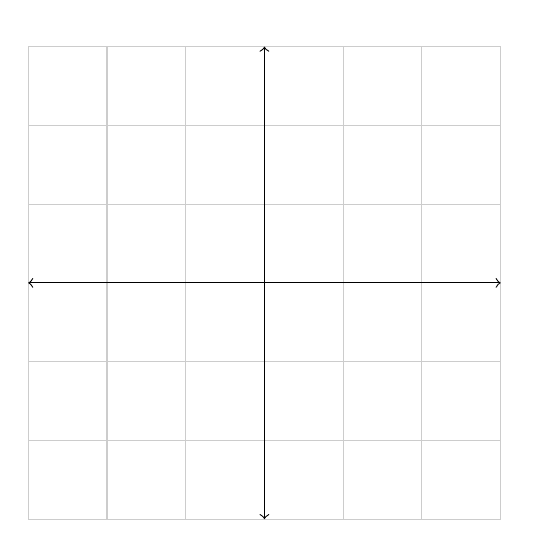
\begin{tikzpicture}
        \draw[thin,gray!40] (-3,-3) grid (3,3);
        \draw[<->] (-3,0)--(3,0) node[right]{$\RE$};
        \draw[<->] (0,-3)--(0,3) node[above]{$\IM$};
        \end{tikzpicture}
        \end{center}
        
        So, for example, let us plot a few points in the complex plane. We'll take
        \[
        z_1=1+i \qquad z_2=-1+i \qquad z_3=2-2i \qquad z_4=-2-i
        \]
        
        \begin{center}
        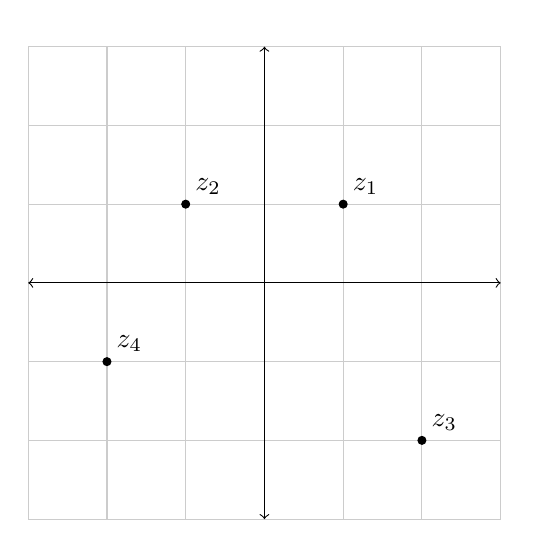
\begin{tikzpicture}
        \draw[thin,gray!40] (-3,-3) grid (3,3);
        \draw[<->] (-3,0)--(3,0) node[right]{$\RE$};
        \draw[<->] (0,-3)--(0,3) node[above]{$\IM$};
       %\addplot+[only marks] coordinates {(1,1) (-1,1) (2,-2) (-2,-1)};
        \foreach \Point/\PointLabel in {(1,1)/z_1, (-1,1)/z_2, (2,-2)/z_3, (-2,-1)/z_4}
        \draw[fill=black] \Point circle (0.05) node[above right] {$\PointLabel$};
        \end{tikzpicture}
        \end{center}
        
        Let us investigate what our algebra was doing geometrically!
        
        \noindent\textbf{Addition of complex numbers:} Recall that if we have $z_1=a_1+b_1 i$ and $z_2=a_2+b_2 i$ then
        \[
        z_1+z_2 = a_1+a_2 + (b_1 +b_2)i.
        \]
        With an explicit example, let us take
        \[
        z_1 = 1+i \qquad z_2=1-2i
        \]
        Then
        \[
        z_3=z_1+z_2=2-i.
        \]
        
        \begin{center}
        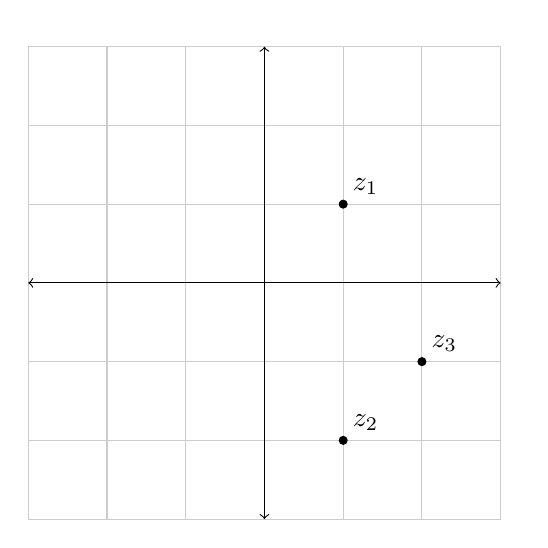
\begin{tikzpicture}
        \draw[thin,gray!40] (-3,-3) grid (3,3);
        \draw[<->] (-3,0)--(3,0) node[right]{$\RE$};
        \draw[<->] (0,-3)--(0,3) node[above]{$\IM$};
       %\addplot+[only marks] coordinates {(1,1) (-1,1) (2,-2) (-2,-1)};
        \foreach \Point/\PointLabel in {(1,1)/z_1, (1,-2)/z_2, (2,-1)/z_3}
        \draw[fill=black] \Point circle (0.05) node[above right] {$\PointLabel$};
        \end{tikzpicture}
        \quad
        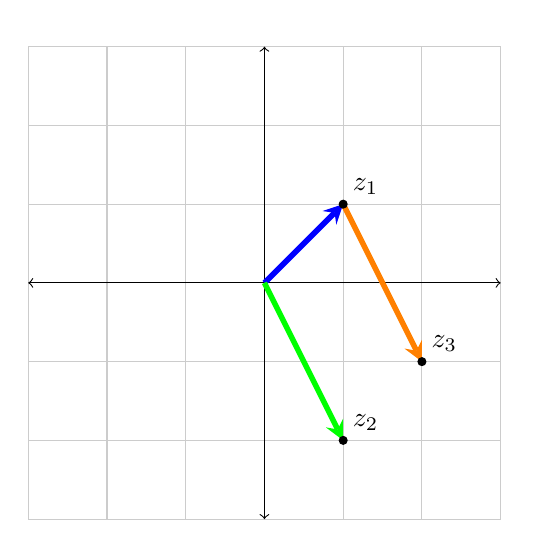
\begin{tikzpicture}
        \draw[thin,gray!40] (-3,-3) grid (3,3);
        \draw[<->] (-3,0)--(3,0) node[right]{$\RE$};
        \draw[<->] (0,-3)--(0,3) node[above]{$\IM$};
        \draw[line width=2pt,blue,-stealth](0,0)--(1,1) node[anchor=east] at (1,1){};
        \draw[line width=2pt,green,-stealth](0,0)--(1,-2) node[anchor=east] at (1,-2){};
        \draw[line width=2pt,orange,-stealth](1,1)--(2,-1) node[anchor=east] at (2,-1){};
        \foreach \Point/\PointLabel in {(1,1)/z_1, (1,-2)/z_2, (2,-1)/z_3}
        \draw[fill=black] \Point circle (0.05) node[above right] {$\PointLabel$};
        \end{tikzpicture}
        \end{center}   
        Geometrically, we arrive at $z_3$ the same way we would do vector addition in the plane $\R^2$.
        
        How about the complex conjugate? What was this doing? Given a complex number $z=a+bi$, we know that $z^*=a-bi$.  So, take the example
        \[
        z=2+2i \qquad z^*=2-2i.
        \]
        \begin{center}
        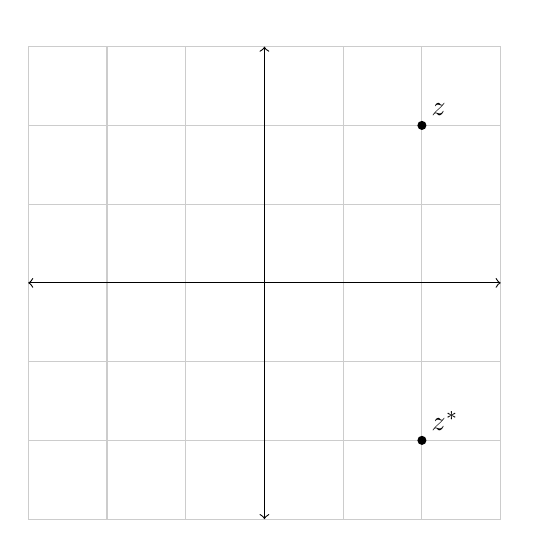
\begin{tikzpicture}
        \draw[thin,gray!40] (-3,-3) grid (3,3);
        \draw[<->] (-3,0)--(3,0) node[right]{$\RE$};
        \draw[<->] (0,-3)--(0,3) node[above]{$\IM$};
       %\addplot+[only marks] coordinates {(1,1) (-1,1) (2,-2) (-2,-1)};
        \foreach \Point/\PointLabel in {(2,2)/z, (2,-2)/z^*}
        \draw[fill=black] \Point circle (0.05) node[above right] {$\PointLabel$};
        \end{tikzpicture}
        \end{center}
        Notice that complex conjugation is just reflection about the real axis!  
        
        \section{Polar coordinates}
        An extremely important notion in planar geometry is that of \emph{polar coordinates}. Usually, we are happy to reference a point in the plane by giving the $x$-coordinates and $y$-coordinates.  In the complex case, we can give the $\RE$ and $\IM$ parts of the complex number to specify its location in the complex plane $\C$.
        
        There are many different ways you could choose to represent points in the plane, but almost all of them are rather silly to a human.  However, one that provides a great bit of intuition is polar coordinates. The idea is as follows:
        
        \begin{df}{Polar Coordinates}{pol_coord}
        \textbf{Polar coordinates} are the a coordinate system that uses $r$, the distance from the origin, and $\theta$, the counter-clockwise angle measured from the $\RE$ axis in the complex plane $\C$ (or $x$-axis in $\R^2$).
        \end{df}
        
        The following image may prove to be helpful.  
        
        \begin{center}
  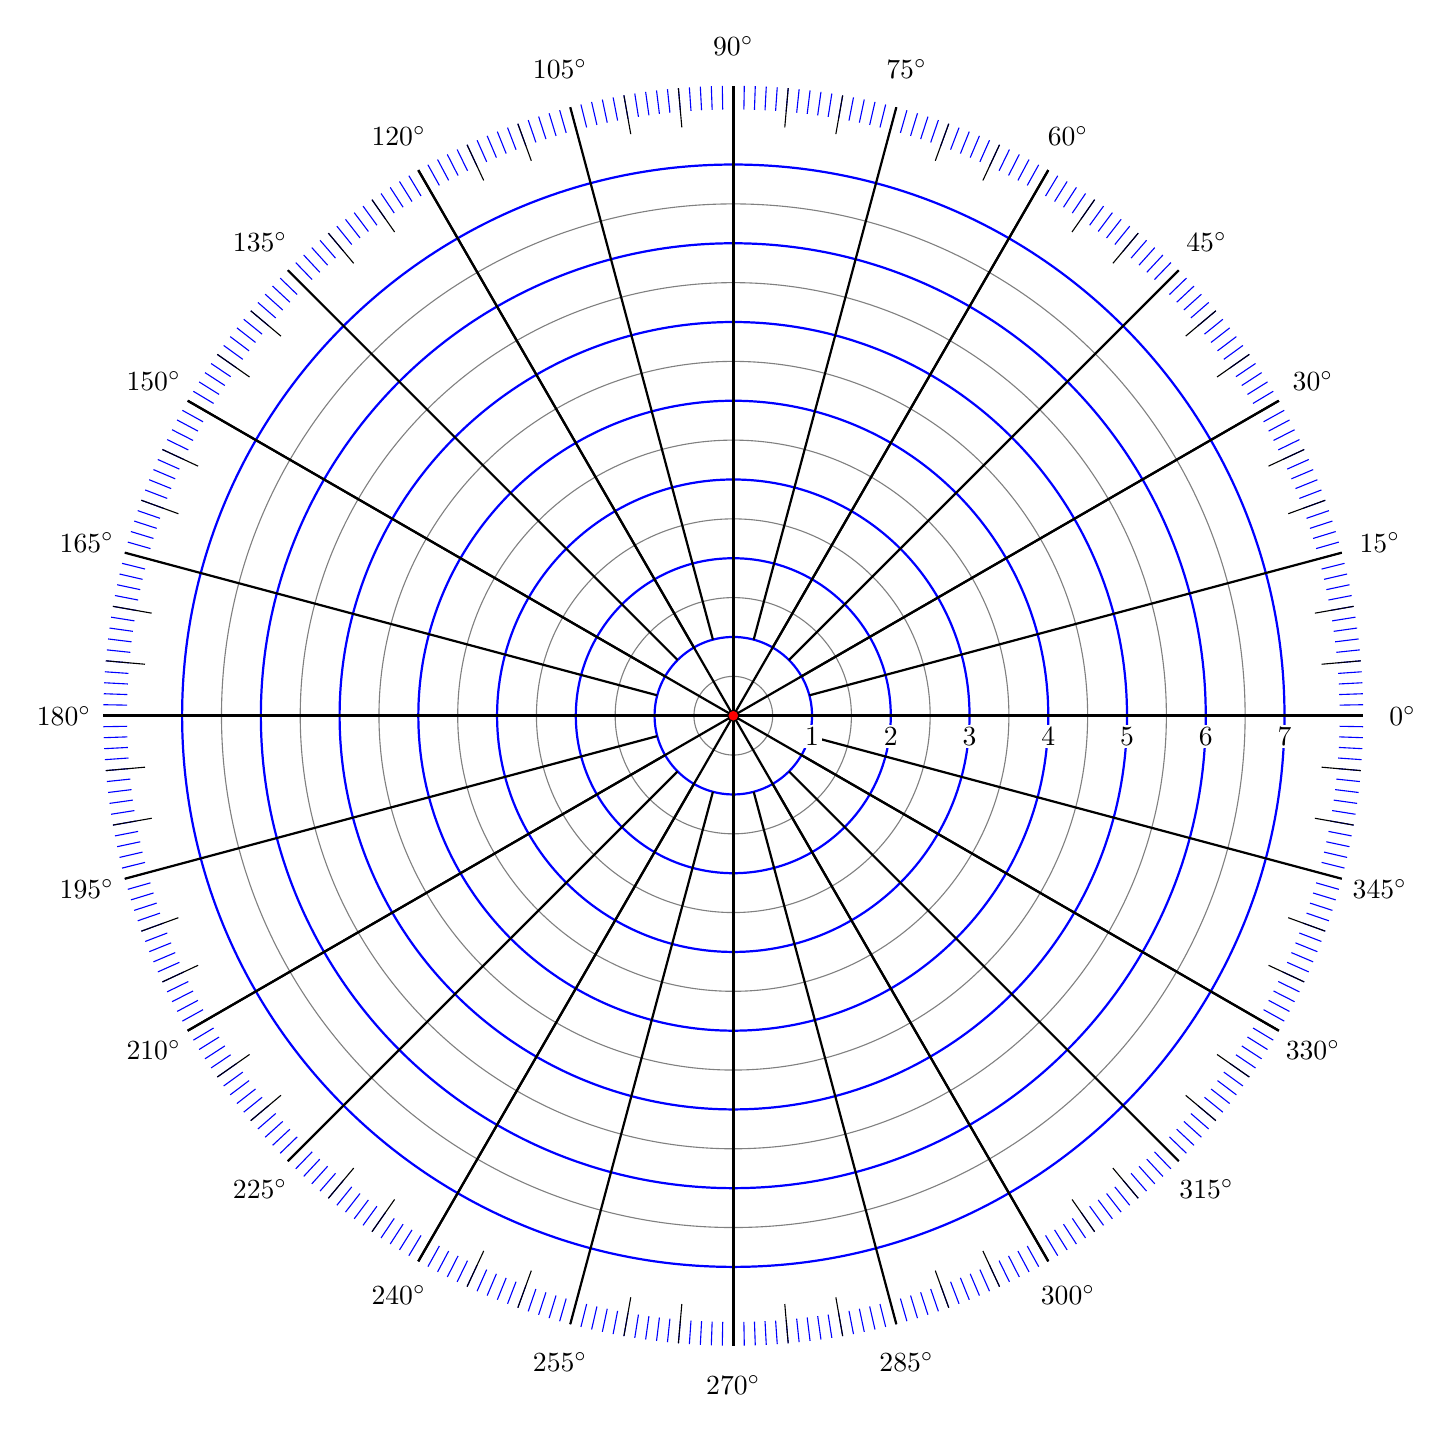
\begin{tikzpicture}
    %Circles 
    \foreach \r in {1, 2,...,7}
      \draw[blue, thick] (0,0) circle (\r);    
    \foreach \r in {0.5, 1.5,...,7}
      \draw[gray, thin] (0,0) circle (\r);
    %1° Rays
    \foreach \a in {0, 1,...,359}
      \draw[blue] (\a:7.7) -- (\a:8);
    %5° Rays
    \foreach \a in {0, 5,...,359}
      \draw[black] (\a:7.5) -- (\a:8);      
    %15° Rays
    \foreach \a in {0, 15,...,359}
      \draw[thick,black] (\a:1) -- (\a:8); 
    %30° Rays
    \foreach \a in {0, 30,...,359}
      \draw[thick,black] (0, 0) -- (\a:8);
    %Radius labels (background filled white)
    \foreach \r in {1, 2,...,7}
      \draw (\r,0) node[inner sep=1pt,below=3pt,rectangle,fill=white] {$\r$};
    %Main rays
    \foreach \a in {0, 90,...,359}
      \draw[very thick] (0, 0) -- (\a:8);
    %Angle labels  
    \foreach \a in {0, 15,...,359}
      \draw (\a: 8.5) node {$\a^\circ$};
    %Central point
    \draw[fill=red] (0,0) circle(0.7mm);
  \end{tikzpicture}
\end{center}
In this picture you can see that coordinates are given by a distance from the origin and an angle.  Of course, we remember that we tend to prefer radians, so in this case we would have
\[
0^\circ = 0 \quad 45^\circ = \frac{\pi}{4} \quad 90^\circ = \frac{\pi}{2} \quad 180^\circ = \pi.
\]

\begin{question}
        If we are given a point in cartesian coordinates (specifying a $\RE$ and $\IM$ part in $\C$ (or $(x,y)$ in $\R^2$), how can we find the polar coordinates $(r, theta)$? How about vice-versa?
\end{question}
        
        We will answer this question, but we need a bit more structure before we can get to it efficiently.
        
        \subsubsection{Taylor Series*}
        $*$ This section is not part of the class but is an extremely important concept.  Fundamentally, functions we care about can be approximated by their derivatives at a single point. For example, take the function $e^x$.  It turns out, we can write this function in a new way.  That is in the form of a \emph{power series}. In fact, we have 
        \[
        e^x = \sum_{n=0}^\infty \frac{x^n}{n!}.
        \]
        More generally, for other functions (with some sufficient conditions I don't care to get into) we can write:
        \[
        f(x)=\sum_{n=0}^\infty \frac{f^{(n)}(c)}{n!}(x-c)^n.
        \]
        The latter is known as the \textbf{Taylor series for $f$ centered at $x=c$}.
        
        You really may wonder why in the world I've just introduced this rather abstract concept, but it plays a fundamental role in the complex world.
        
        \subsubsection{Euler's Formula}
        Using the above Taylor series for $e^x$, we can plug in the following:
        \[
        e^{i\theta}=\sum_{n=0}^\infty \frac{(i\theta)^n}{n!}.
        \]
        It turns out that we find
        \[
        e^{i\theta} = \cos \theta + i \sin \theta.
        \]
        This result is known as \textbf{Euler's formula}. 
        
        \subsubsection{Polar Coordinates in $\C$}
        It turns out that Euler's formula gives us all the necessary tools to represent numbers in the complex plane in a cartesian or polar way.  
        
        \begin{df}{Modulus}{modulus}
        Given a complex number $z$, the \textbf{modulus} $\|z\|$ (think \emph{length}) of a complex number is given by
        \[
        \|z\|=\sqrt{zz^*}.
        \]
        Letting $z=a+bi$ we find
        \[
        \|z\|=\sqrt{a^2+b^2},
        \]
        which is not entirely shocking.  Just like the lengths of vectors in the plane, the ``length" of a complex number follows suit.
        \end{df}
        
        \begin{question}
                Given any $\theta$, what is the modulus of $z=e^{i\theta}$?
        \end{question}
        
        \begin{answer}
        We take
        \[
        z=e^{i\theta}=\cos \theta + i \sin \theta.
        \]
        Then
        \[
        zz^*=\cos^2 \theta + \sin^2 \theta = 1.
        \]
        So
        \[
        \|z\|=\sqrt{1}=1.
        \]
        \end{answer}
        
        It turns out that there is a fundamental relationship underlying the complex numbers.  The moral of the story is that imaginary parts of complex numbers cause rotations while the real parts cause scaling. This isn't entirely the case, but it's an alright analogy. We'll be able to uncover this as we explore polar coordinates in more depth.
        
        \subsubsection{Coordinate systems}
        \begin{remark}
        Something should be said here about the idea of coordinates in general.  Points in a plane are just that -- points.  Where they are located relative to each other is the fundamental structure whereas how we choose to measure this distance is not.  
        
        Polar coordinates are just another way of specifying where a point is located.  This choice of coordinates should not change the behavior of the algebra we have developed or any of the geometry.  Does choosing to measure an object in inches versus centimeters change the length of the object? Of course not.
        \end{remark}
        
        \section{Euler's formula and polar coordinate transformations}
        The fact that we can write
        \[
        e^{i\theta}= \cos \theta + i \sin \theta
        \]
        means that we can control the angle of a line that the complex number lives on.  Since the above function lies on the unit circle in $\C$, we can scale this with a real number to reach any point in $\C$. 
        
        That is, an equivalent way to represent a point in $\C$ is to specify its \textbf{argument} (angle, denoted $\arg(z)$) $\theta$ and its \textbf{modulus} (distance from the origin, denoted $r$ or $\|z\|$) $r$ and write
        \[
        z=re^{i\theta}.
        \]
        Before, we had always written this in a cartesian way, like
        \[
        z=a+bi.
        \]
        But we also have Euler's formula, which means that
        \[
        a+bi = re^{i\theta} = r\cos \theta + i r \sin \theta.
        \]
        This means that
        \[
        a=r\cos \theta
        \]
        and 
        \[
        b = r \sin \theta.
        \]
        You can also see that this is really nothing more than the pythagorean theorem and trigonometry the following figure.
        \begin{figure}[H]
            \centering
            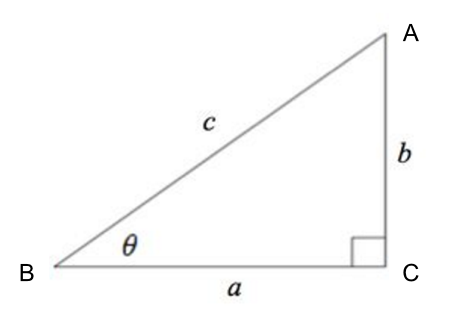
\includegraphics[width=.4\textwidth]{Figures/triangle_theta.png}
        \end{figure}
        In this case, the length of the hypotenuse ($c$ in the figure) is given by $r$. 
        
        \noindent \textbf{\textbf{Conversion from polar to cartesian:}} If you're given a point in $\C$ in polar coordinates,
        \[
        z=re^{i\theta},
        \]
        then in cartesian coordinates it will read
        \[
        z=r\cos \theta + ir\sin \theta.
        \]
        This is
        \[
        a=r\cos \theta \qquad b=r\sin \theta.
        \]
        
        \noindent \textbf{\textbf{Conversion from cartesian to polar:}} If you're given a point in $\C$ is cartesian coordinates,
        \[
        z=a+bi,
        \]
        then in polar coordinates it will read
        \[
        z=\|z\|e^{i\arctan(b/a)}.
        \]
        That is that the modulus and argument follow
        \[
        r = \|z\|=\sqrt{zz^*} \qquad \theta = \arctan\left( \frac{b}{a}\right)
        \]
        respectively. We defined $\|z\|$ to be the distance $z$ is from the origin, so this is clear.  The $\arctan(b/a)$ can be realized from the trigonometric fact that
        \[
        \tan \theta = \frac{b}{a}
        \]
        and inverting.
        
        
        \section{Multiplication of complex numbers}
        
        While we were perfectly happy to multiply complex numbers in cartesian form, it is more illuminating to multiply them in polar form.  Let us take two complex numbers
        \[
        z_1 = r_1 e^{i\theta_1} \qquad z_2 = r_2 e^{i\theta_2}.
        \]
        Then we can write the product:
        \[
        z=z_1 z_2 = (r_1 e^{i\theta_1})(r_2 e^{i\theta_2})= r_1r_2 e^{i(\theta_1+\theta_2)}.
        \]
        The thing to notice here is that the modulus of a product follows
        \[
        \|z\|=\|z_1\|\|z_2\|=r_1r_2
        \]
        and the argument of a product follows
        \[
        \arg(z)=\arg(z_1)+\arg(z_2).
        \]
        All of this is to say to the following: Multiplication of complex numbers is decomposed into rotation and scaling.
    
    
        \subsubsection{Multiplicative inverse in polar form}
        We found before that given a complex number $z$, we can find the multiplicative inverse $z^{-1}=1/z$ in cartesian form.  But this was a bit of a headache.  In polar form, however, it is much easier.  Recall that if we have
        \[
        z_1 z_2 = \left(r_1e^{i\theta_1}\right)\left(r_2e^{i\theta_2}\right)=r_1r_2e^{i(\theta_1+\theta_2)}.
        \]
        
        Now, given $z=re^{i\theta}$ we can find fairly quickly that $z^{-1}$ must be
        \[
        z^{-1}=\frac{1}{r}e^{-i\theta}.
        \]
        
        \begin{exercise}
        Show that this is indeed the multiplicative inverse.
        \end{exercise}
        
        \section{Complex functions}
        Up until now we have just looked at complex numbers themselves.  But, just having the number structure is not so interesting.  We want to investigate a bit of functions of complex numbers.  That is, functions of the form
        \[
        f\colon \C \to \C.
        \]
        These are functions that have a complex number as an input and a complex number as an output. 
        
        \begin{remark}
        Since both the input for $f$ are (essentially) 2-dimensional, we lose the ability to easily visualize these functions as we do in the case of real numbers.  We are then forced to rely more on the algebra.
        \end{remark}
        
        Let us investigate a few complex functions.  
        
        \begin{ex}{Identity Function}{id_func}
        Consider the function $f\colon \C \to \C$ given by $f(z)=z$.  This function takes in a complex number and outputs the same complex number.  So, points in the plane do not move with this function.
        \end{ex}
        
        \begin{ex}{Square Function}{square_func}
        Consider now $g\colon \C \to \C$ given by $g(z)=z^2.$ It's more englightening to write $z$ in polar form with this function.  Let us see why.
        
        Take $z=re^{i\theta}$.  Then
        \[
        g(z)=z^2=\left( re^{i\theta}\right)^2=r^2e^{2i\theta}.
        \]
        We can see that the modulus of the output grows by the square of the modulus of the input.  The argument is simply doubled.  
        \end{ex}
        
        \begin{exercise}
        Take
        \[
        z_1=1+1i \qquad z_2=e^{2\pi/3} \qquad z_3=4 \qquad z_4=-3+2i 
        \]
        as inputs to the squaring function $g$ above.  Find where $g$ outputs these inputs.
        \end{exercise}
        
        There is a lot more to say about complex functions, but it takes far more tools and time than we have to spare.
        
        \section{Contours}
        One specific example of complex functions we can visualize are \textbf{contours} (or curves).  These are also very useful and we will extend the notion of contours to curves in space.
        
        What is a contour?  It is a function of the form
        \[
        \gamma \colon \R \to \C.
        \]
        That is, $\gamma$ takes in a real number input, and outputs a complex number.  These functions look like curves in the plane.  Let's visit an example.
        
        \begin{ex}{Line Contour}{line_cont}
        Let us consider the contour
        \[
        \gamma(t)=t+it.
        \]
        Then we find that $\gamma$ looks like the $y=x$ line we write in the plane.
        
        \begin{center}
            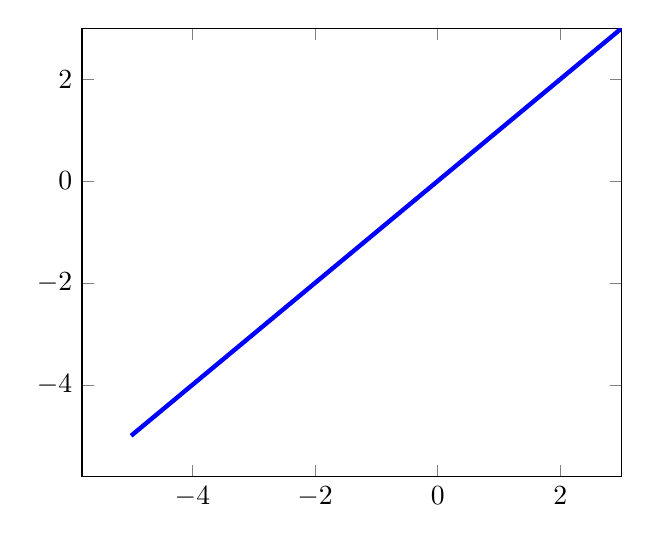
\begin{tikzpicture}
\begin{axis}[xmax=3,ymax=3, samples=50]
  \addplot[blue, ultra thick] (x,x);
\end{axis}
\end{tikzpicture}
        \end{center}
        \end{ex}
        
        \begin{ex}{Circle Contour}{circ_cont}
        Consider the contour given by
        \[
        \gamma(t)=2e^{2\pi i t}.
        \]
        Then we find that the contour is a circle with radius 2 centered at the origin.
        \begin{figure}[H]
            \centering
            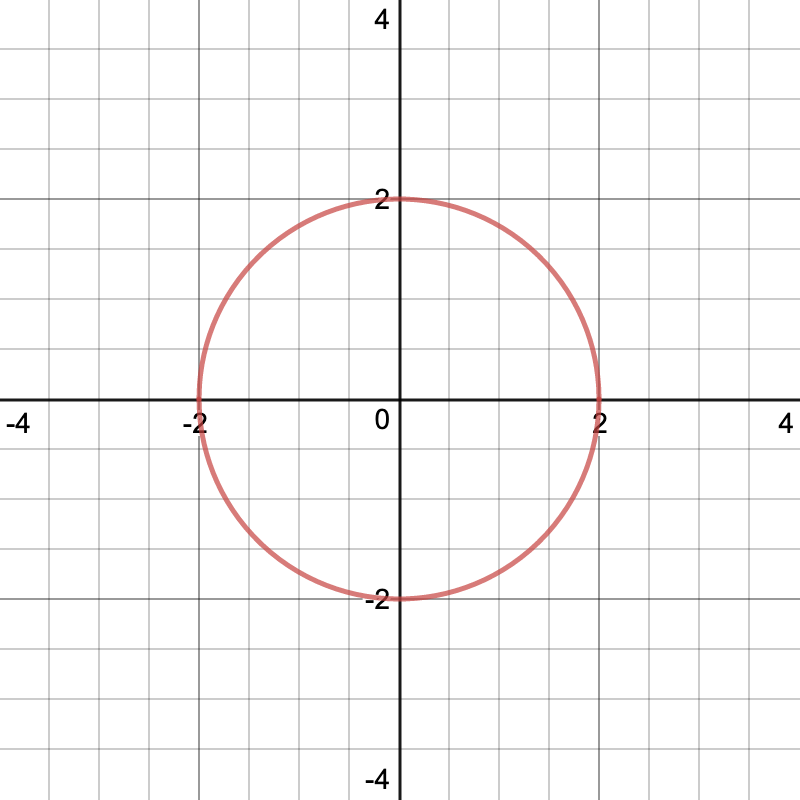
\includegraphics[width=.4\textwidth]{Figures/circle_r2.png}
        \end{figure}
        \end{ex}
        
        Up to this point, we have not really done any calculus.  But this will change now! We can ask a few questions about contours.  One in particular is the \textbf{velocity} $\gamma'(t)$ at a point in time $t$.  The other question we will look at has to do with adding up function values along a contour in the form of a \textbf{contour integral}.  These ideas will extend to higher dimensions nicely.  
        
        \section{Derivatives of contours}
        
        \begin{df}{Velocity of a Contour}{vel_cont}
        The \textbf{velocity} (or \textbf{tangent}) at time $t$ to a contour $\gamma \colon [a,b] \to \C$ is $\gamma'(t)$. That is,
        \[
        \gamma'(t)=\frac{d\gamma}{dt}=\lim_{\delta\to 0} \frac{\gamma(t+\delta)-\gamma(t)}{\delta}.
        \]
        \end{df}
        
        \begin{ex}{Velocity on a Line}{vel_on_line}
        If we take $\gamma \colon \R \to \C$ given by
        \[
        \gamma(t)=t+it,
        \]
        then the tangent is
        \begin{align*}
        \gamma'(t)&=\lim_{\delta \to 0} \frac{\gamma(t+\delta)-\gamma(t)}{\delta}\\
        &=\lim_{\delta \to 0} \frac{(t+\delta)+(t+\delta)i-t-it}{\delta}\\
        &= \lim_{\delta \to 0} \frac{\delta + i\delta}{\delta}\\
        &= 1+i.
        \end{align*}
        Doing this limit isn't necessary each time.  Instead, you should use the derivative rules you already know to do this.  You just have to do this in two parts and use the \emph{sum rule} and \emph{constant multiple rule} for derivatives in this case. 
        
        Take
        \[
        \frac{d}{dt}(t+it)=\frac{d}{dt}(t)+i\frac{d}{dt}(t)=1+i.
        \]
        \end{ex}
        
        \begin{ex}{Velocity on a Circle}{vel_on_circ}
        Consider the contour $\gamma \colon [0,1] \to \C$ given by
        \[
        \gamma(t)=2e^{2\pi i t}.
        \]
        You can imagine this as a particle orbiting a mass placed at the origin.  Then the velocity at a time $t$ is
        \[
        \gamma'(t)=4\pi i e^{2\pi i t}. 
        \]
        We can in fact find the \emph{acceleration} if we'd like.  Just take
        \[
        \gamma''(t)=-8\pi^2 e^{2\pi i t}.
        \]
        Just as a sanity check, you can check this against the centripetal acceleration magnitude you see in a physics course which is
        \[
        a=\frac{v^2}{r}.
        \]
        Here we find
        \[
        \frac{v^2}{r}=\frac{(4\pi i )^2}{2}=-8\pi^2=a.
        \]
        \end{ex}
        
        \begin{exercise}
        Draw the circle contour and draw the velocity and acceleration at the points $t=0$, $t=1/4$, $t=1/2$, and $t=3/4$. 
        \end{exercise}
        
        \section{Integration of contours}
        Many times we choose contours since we only care about a particle traveling through a region.  We just saw how we can find the velocity of the particle, but if we want to ``add up" the values of a complex valued function $f\colon \C \to \C$ we need to have some notion of integration.
        
        \begin{df}{Contour Integral}{cont_int}
        Given a complex function $f\colon \C \to \C$ and a contour $\gamma \colon [a,b] \to \C$, the \textbf{contour integral of $f$} is
        \[
        \int_\gamma f(\gamma)d\gamma.
        \]
        Now, $\gamma$ is a function of $t$, and we can write using a change of variables
        \[
        \int_\gamma f(\gamma)d\gamma = \int_a^b f(\gamma(t))\gamma'(t)dt.
        \]
        This is now something we know how to integrate.
        \end{df}
        
        \begin{ex}{Contour Integral on a Line}{cont_int_on_line}
        Let $f(z)=2+i$ and $\gamma(t)=t+it$.  Then we can integrate this contour from $t=0$ to $t=1$ by
        \begin{align*}
        \int_\gamma f(\gamma)d\gamma &= \int_0^1 f(t+it)(1+i)dt\\
        &= \int_0^1 (2+i)(1+i)dt\\
        &=(1+3i)\int_0^1 dt\\
        &=(1+3i).
        \end{align*}
        \end{ex}
        
        \begin{ex}{Contour Integral on a Circle}{cont_int_on_circ}
        Let $f(z)=z^2$ and $\gamma(t)=e^{2\pi i t}$. Then we can integrate this contour from $t=0$ to $t=1$ by
        \begin{align*}
            \int_\gamma f(\gamma)d\gamma &= \int_0^1 f\left(e^{2\pi i t}\right) (2\pi i)dt\\
            &= 2\pi i \int_0^1 \left(e^{2\pi i t}\right)^2 dt\\
            &= 2\pi i \int_0^1 e^{4\pi i t} dt.
        \end{align*}
        Here we need to use a substitution that $u=4\pi i t$ and $du=4\pi i dt$ which gives us that $u=0$ when $t=0$ and $u=4\pi i$ when $t=1$
        \begin{align*}
            \int_\gamma f(\gamma)d\gamma &= \frac{1}{2}\int_0^{4\pi i} e^u du\\
            &= \frac{1}{2} \left[ e^u \right]_0^{4\pi i}=0.
        \end{align*}
        This is zero since
        \[
        e^{4\pi i t}=e^0=1.
        \]
        \end{ex}
        
        \begin{exercise}
        Let $f(z)=z^2$ and $\gamma(t)=1+it^2$.  Then evaluate the contour integral from $t=0$ to $t=1$.
        \end{exercise}
        
        
        \chapter{Multivariable Functions}
        
        \section{Overview of multivariate functions}
        Now that we have covered enough of the complex numbers, we will move back into the vector space $\R^n$ and analyze the types of functions we can have with this space.  Specifically, we will concentrate on $\R^3$ (or $\R^2$) and functions of the form:
        \begin{align}
            &\gamma\colon \R \to \R^3\\
            &f\colon \R^3 \to \R\\
            &\mathbf{v}\colon \R^3 \to \R^3.
        \end{align}
        Abstractly, I could call each one of these functions a \emph{field} (in the physics sense).  However, I'll refrain from this (and let the mathematicians breathe a sigh of relief).
        
        
        \begin{enumerate}[(1)]
        \item Functions of the form
        \[
        \gamma \colon \R\to \R^3
        \]
        are \textbf{curves}.  Often times, we will have 
        \[
        \gamma \colon [a,b]\to \R^3
        \]
        when we want curves with specific endpoints. We will concentrate first on curves, so I'll save the extra detail for a bit later.
        
        \item Functions of the form
        \[
        f\colon \R^3 \to \R
        \]
        are \textbf{scalar fields} or \textbf{scalar functions}.   These functions are useful in describing quantities like temperature in space.  At each point in space $\R^3$, we can assign a single number $\R$ that tells us this temperature.  One may ask how this function changes from point to point.  Asking this question sends you immediately to investigating the \emph{gradient}.  It turns out, using our temperature example, that we can understand heat flow by understanding temperature gradients.
        
        \item Functions of the form
        \[
        \mathbf{v}\colon \R^3 \to \R^3
        \]
        are called \textbf{vector fields}.  Roughly speaking, at each point in space $\R^3$, we can place a vector that is also in $\R^3$.  These fields are very important in describing systems that have flow.  For example, fluid flow or electromagnetism are vector field theories.  What will it mean to find the change in a vector field?  This will lead us to the notion of the \emph{total derivative}.  This concept is a bit abstract at first but will really tell us the proper notion of the derivative.
        \end{enumerate}
        
        \section{Curves in space}
        
        We will begin these multivariate functions by considering functions that are not multivariate!  Why? Because curves are very much useful tools and this will help us visualize results for the other types of functions.
        
        Let us consider a curve
        \[
        \gamma \colon \R \to \R^3.
        \]
        We will specify a specific curve by supplying three functions $f_1(t)$, $f_2(t)$, and $f_3(t)$. Specifically, each of these functions $f_i$ is a function $f_i\colon \R \to \R$. Then, we can say that
        \[
        \gamma(t)=(f_1(t),f_2(t),f_3(t))=\begin{bmatrix} f_1(t)\\ f_2(t)\\ f_3(t)\end{bmatrix}.
        \]
        \emph{Note, I will likely use these above notations for vectors interchangeably.} 
        
        Each $f_i(t)$ (for the values $i=1,2,3$) is called a \textbf{coordinate function}.  Intuitively, the coordinate function tells us where the curve is at a time $t$. That is
        \begin{align*}
            &f_1(t) \quad \textrm{the $x$-position of $\gamma$ at time $t$,}\\
            &f_2(t) \quad \textrm{the $y$-position of $\gamma$ at time $t$,}\\
            &f_3(t) \quad \textrm{the $z$-position of $\gamma$ at time $t$.}
        \end{align*}
        The nice thing about these coordinate functions is we entirely know how to deal with their calculus since each is a function $f_i\colon \R \to \R$.
        
        Now, we can find the \textbf{tangent vector} or \textbf{velocity vector} to the curve $\gamma$ at a time $t$.  We covered this in the complex case, and the idea here is arguably more straightforward. 
        
        Imagine that $\gamma(t)$ is the position of a small particle at the time $t$.  Then the velocity is the time rate of change of this position.  Specifically, we see how each of the coordinate functions changes, and this will tell us how the position changes! So, we have the following.
        
        \begin{df}{Tangent Vector to a Curve}{tang_to_curve}
        Given a curve $\gamma$, the \textbf{tangent vector to $\gamma$ at the time $t$} is
        \[
        \gamma'(t)=\lim_{\delta \to 0} \frac{\gamma(t+\delta)-\gamma(t)}{\delta}.
        \]
        It turns out that we find $\gamma'$ is
        \[
        \gamma'(t)=(f_1'(t),f_2'(t),f_3'(t))=\begin{bmatrix} f_1'(t)\\ f_2'(t)\\ f_3'(t)\end{bmatrix}.
        \]
        \end{df}
        
        \begin{ex}{Graph of a Quadratic Function}{graph_quad}
        Consider the curve $\gamma\colon \R \to \R^2$ given by
        \[
        \gamma(t)=(t,t^2).
        \]
        This curve looks exactly like the graph of the function $f(x)=x^2$ that we have drawn many times before. 
        \begin{figure}[H]
            \centering
            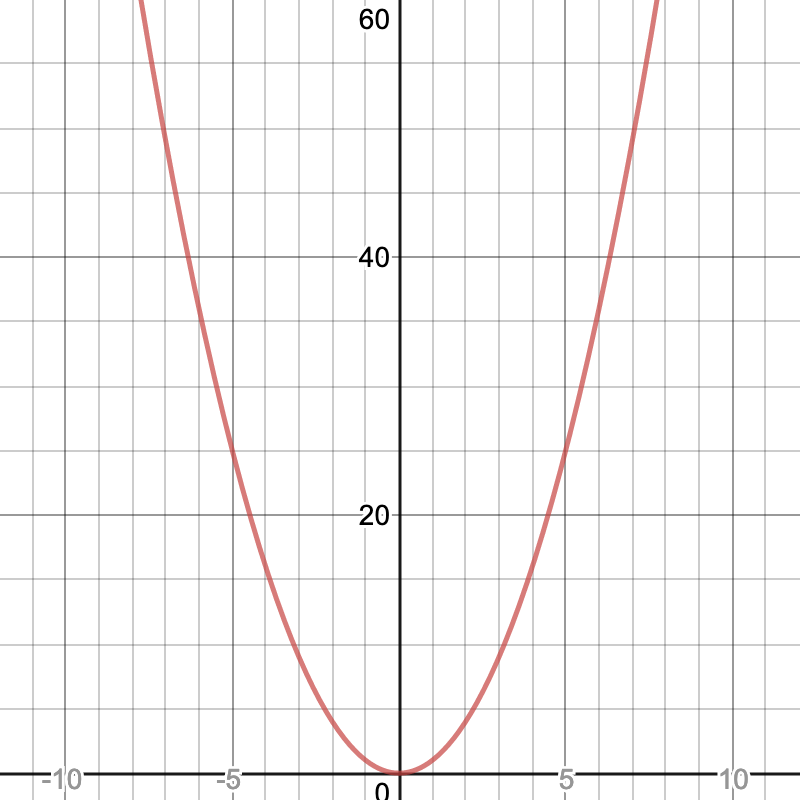
\includegraphics[width=.4\textwidth]{Figures/quadratic_curve.png}
        \end{figure}
        
        What is the tangent vector at time $t$? We have
        \[
        \gamma'(t)=(1,2t).
        \]
        If we take this $y$-value over the $x$-value we arrive at the same conclusion for the derivative to $f(x)=x^2$ (i.e., $f'(x)=2x$).
        \end{ex}
        
        \begin{ex}{Circle Curve}{circ_curve}
        Consider the curve $\gamma \colon [0,1] \to \R^2$ given by
        \[
        \gamma(t)=(\cos (2\pi t),\sin (2\pi t)).
        \]
        This curve is a circle of radius $1$ centered at $(0,0)$.  We can find the tangent vector at a time $t$ by
        \[
        \gamma'(t)=(-2\pi \sin(2\pi t), 2\pi \cos(2\pi t)).
        \]
        See the following graphs
        
    \begin{figure}[H]
    \centering
    \begin{subfigure}[h]{0.45\textwidth}
        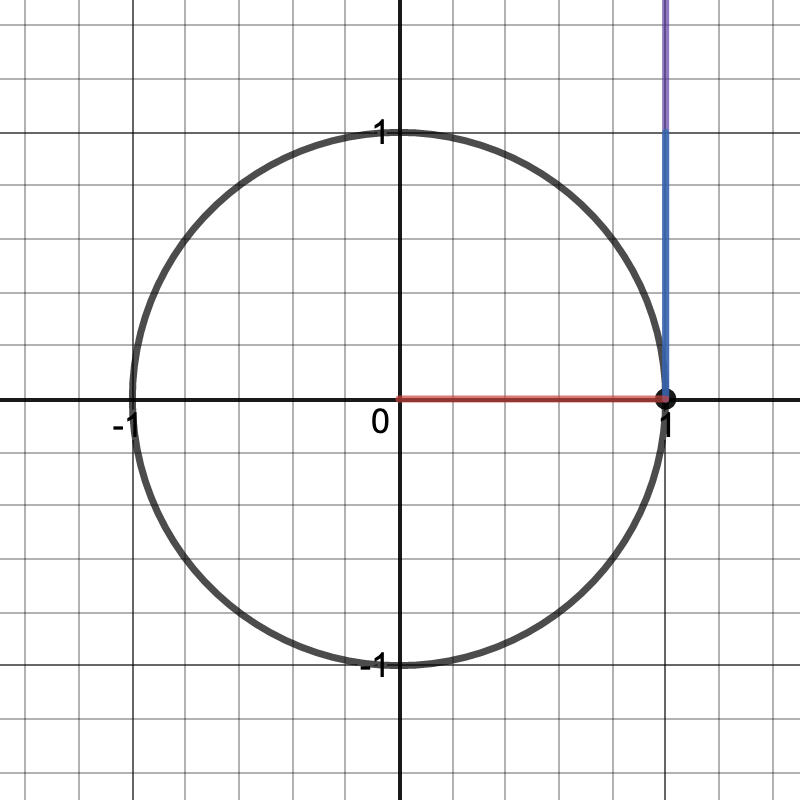
\includegraphics[width=\textwidth]{Figures/circ_tang_1.png}
        \caption{Tangent vector at $t=0$.}
    \end{subfigure}
    ~ 
    \begin{subfigure}[h]{0.45\textwidth}
        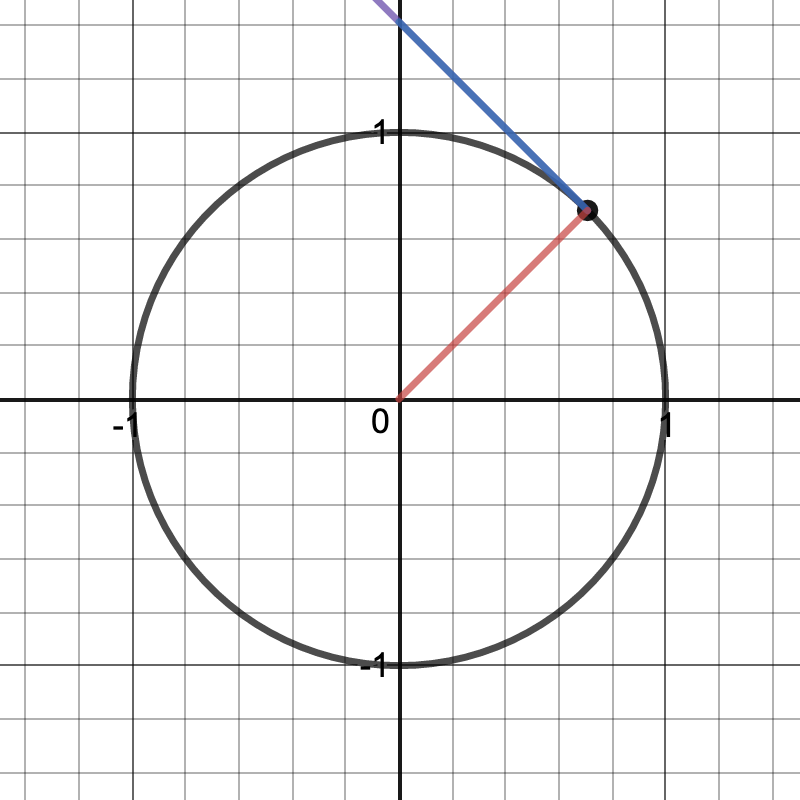
\includegraphics[width=\textwidth]{Figures/circ_tang_2.png}
        \caption{Tangent vector at $t=\frac{1}{8}$.}
    \end{subfigure}
    
    \begin{subfigure}[h]{0.45\textwidth}
        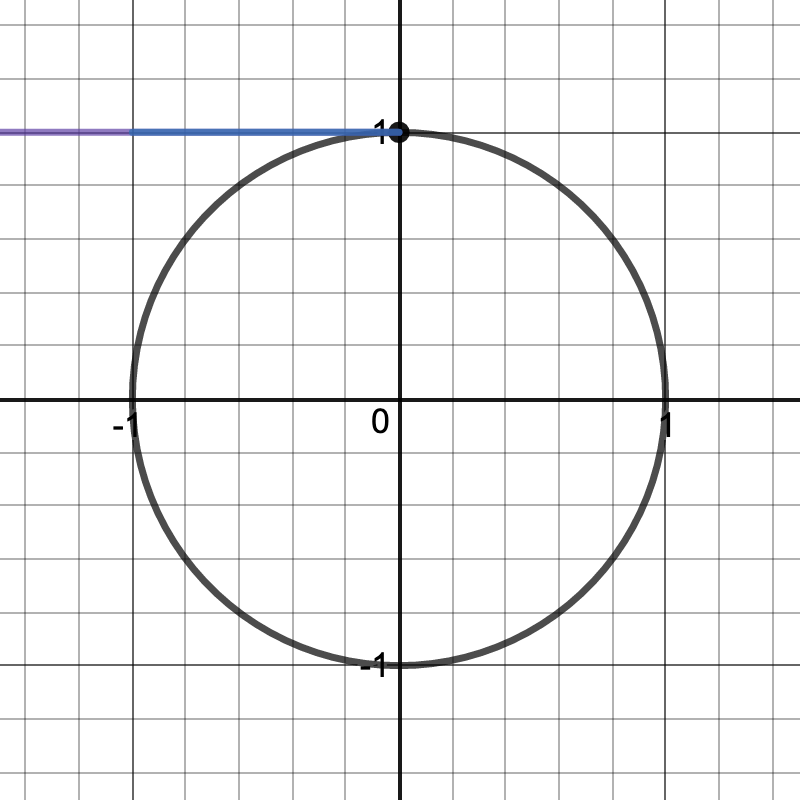
\includegraphics[width=\textwidth]{Figures/circ_tang_3.png}
        \caption{Tangent vector at $t=\frac{1}{4}$.}
    \end{subfigure}
    ~
    \begin{subfigure}[h]{0.45\textwidth}
        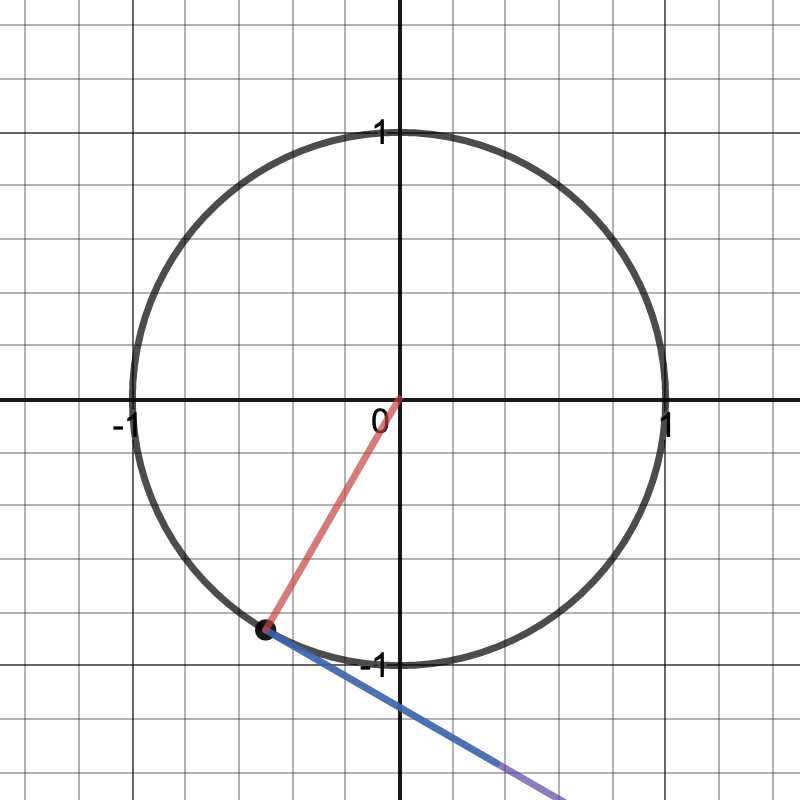
\includegraphics[width=\textwidth]{Figures/circ_tang_4.png}
        \caption{Tangent vector at $t=\frac{2}{3}$.}
    \end{subfigure}
        \end{figure}
        
        We can also compute the \textbf{normal vector} or \textbf{acceleration vector} to a curve by taking another derivative.  We write
        \[
        \gamma''(t)=(-4\pi^2 \cos(2\pi t),-4\pi^2 \sin(2\pi t)).
        \]
        \end{ex}
        
        \subsubsection{Line integrals}
        
        In reality, we like to add up function values along curves.  We have already done this before in the complex case with contours.  You also did this in a calculus I course via the Riemann integral.  We will get to this, but we need to know the correct functions to add up along a curve first. These will be the vector and scalar fields fields.
        
        
        
        \section{Scalar fields}
        The next major class of functions we will consider are the scalar fields.  That is, functions that take the form
        \[
        f\colon \R^3 \to \R.
        \]
        Often, it will be helpful to visualize functions by considering instead
        \[
        f\colon \R^2 \to \R
        \]
        and looking at the \emph{graph} of $f$.  
        
        \begin{ex}{Graph of a function}{graph_of_func}
        Whenever we talk of a function of the form
        \[
        f\colon \R \to \R
        \]
        we inherently tend to draw the graph of the function $f$.  By graph, I mean that given $f$, we usually just draw $(x,f(x))$ in the plane.
        
        Take for example, $f\colon \R \to \R$ given by $f(x)=x^2$.  We usually draw the plane $\R^2$ and graph the curve $(x,f(x))$ which looks like
        \begin{figure}[H]
            \centering
            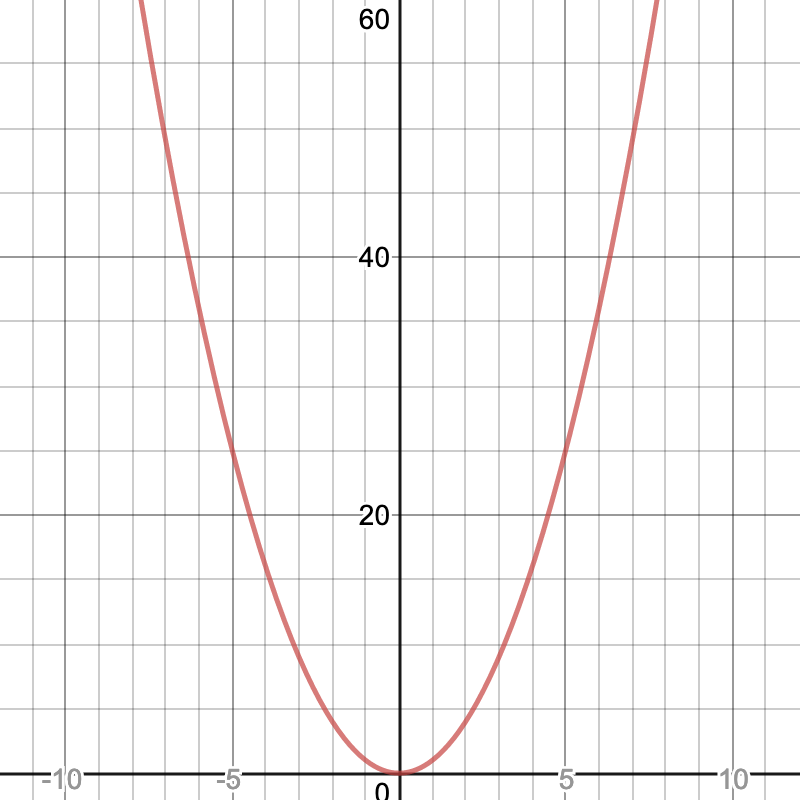
\includegraphics[width=.5\textwidth]{Figures/quadratic_curve.png}           
        \end{figure}
        All of this is to say that graphs of these types of functions are special kinds of curves.  In other words, they are curves that pass the vertical line test.
        \end{ex}
        
        \begin{ex}{The Paraboloid}{paraboloid}
        Let $f\colon \R^2 \to \R$ be given by
        \[
        f(x,y)=x^2+y^2.
        \]
        We can plot the graph of the function by plotting $(x,y, f(x,y))$ in $\R^3$.  This will look like:
        \begin{figure}[H]
            \centering
            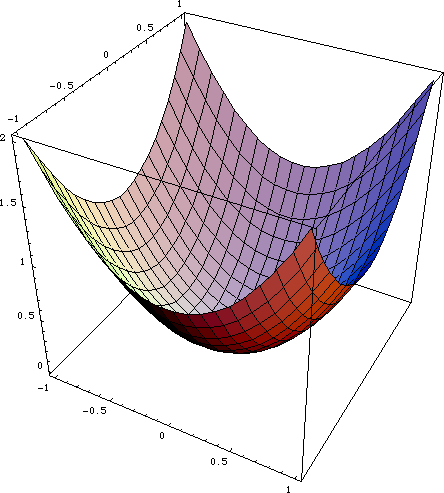
\includegraphics[width=.4\textwidth]{Figures/paraboloid.png}
        \end{figure}
        Then we can analyze this function in a few nice ways.  
        
        If we fix a value for $x$ or $y$, then we will be able to look at $f$ as a function of just a single variable.  
        \begin{itemize}
        \item So we can, for example, fix $y=0$ and then we have
        \[
        f(x,0)=x^2.
        \]
        So along the $y=0$ line, the function is just the parabola we are used to! 
        
        \item Similarly, we can force $x=0$ and arrive at
        \[
        f(0,y)=y^2
        \]
        is also a parabola.  
        
        \item But we are not limited to these choices.  We could have chosen $y=5$ and we would have
        \[
        f(x,5)=x^2+25
        \]
        which is a parabola shifted upwards by 25 units.
        
        \item  Again, we could also choose yet another ``slice" of this function and let $x=y$ which would give us
        \[
        f(x,x)=x^2+x^2=2x^2.
        \]
        So, along the $x=y$ line, the parabola is scaled by 2.
        
        \item One other method of analyzing this function would be to find what the \textbf{level curves} of this function are.  What are the points $(x,y)$ that satisfy $f(x,y)=c$?  We call these level curves much in the way that a topographical map plots curves along the areas with equal height.  For this example, consider the set of points $(x,y)$ so that $f(x,y)=1.$ This means
        \[
        f(x,y)=1=x^2+y^2.
        \]
        Since we have
        \[
        x^2+y^2=1
        \]
        that means each level curve is a circle!
        \item Here is a ``topographical map" for this function (i.e., a plot of the level curves for this paraboloid.)
        \begin{figure}[H]
            \centering
            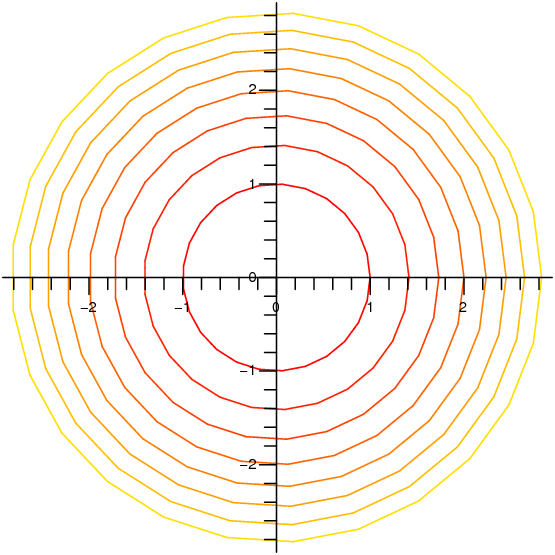
\includegraphics[width=.4\textwidth]{Figures/parabolic_level_curves.png}
        \end{figure}
        Here, each circle represents $f(x,y)=c$ for different values of $c$.  This really \emph{is} a topographical map!
        \end{itemize}
        \end{ex}
        
        \begin{exercise}[Plane]
        Repeat this analysis for yourself for the following function:
        \[
        f(x,y)=x+y.
        \]
        \end{exercise}
        
        \section{Level surfaces}
        In the planar case, we would often have to specify a set of points like
        \[
        x^2+y^2=1
        \]
        which is the circle.  
        
        In higher dimensions, we can do the same in order to visualize functions of the form $f\colon \R^3\to \R$ written as $f(x,y,z)$.  If we pick some constant $c$ and write
        \[
        f(x,y,z)=c
        \]
        then we will get the \textbf{level surfaces} for the function $f(x,y,z)$.  Visualizing functions of three variables (or more) $f(x,y,z)$ requires us to visualize in four or more dimensions. So we often reduce the problem to visualizing level surfaces.
        
        \begin{ex}{A Sphere as a Level Surface}{sphere_lev_surf}
        We can consider the following function
        \[
        f(x,y,z)=x^2+y^2+z^2.
        \]
        If we take the one level set, that is the points $(x,y,z)$ that satisfy
        \[
        x^2+y^2+z^2=1
        \]
        then we get the \emph{2-sphere}.  These are the set of points that are all a distance one from the origin.  Here is a picture:
        \begin{figure}[H]
            \centering
            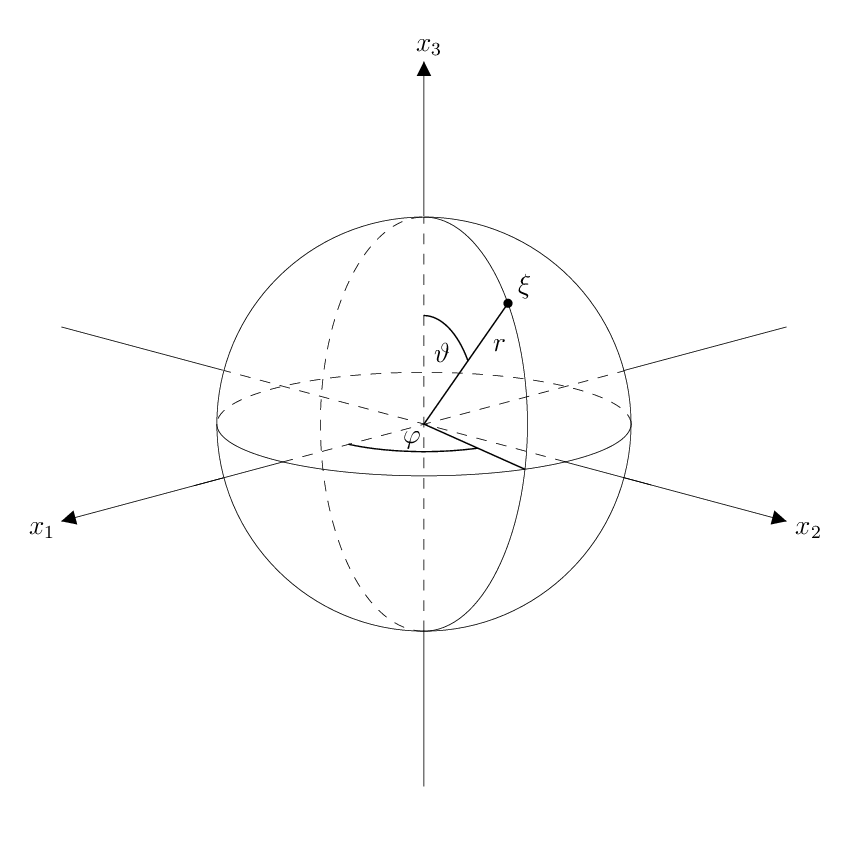
\includegraphics[width=.4\textwidth]{Figures/sphere.png}
        \end{figure}
        \end{ex}
        
        \begin{ex}{The Hyperboloids}{hyperboloids}
        Consider a family of surfaces given by the level surfaces of
        \[
        f(x,y,z)=x^2+y^2-z^2.
        \]
        \begin{itemize}
            \item If we take $c=0$ and set
            \[
            x^2+y^2-z^2=0.
            \]
            then we find the 0 level surface. In this case, we can do a bit of work to find
            \[
            z=\pm \sqrt{x^2+y^2}.
            \]
            Notice, if we pick any value for $z$, that we get a circle at that level!  When $z=0$, we get a single point.  It turns out that we get the \emph{(double) cone} surface which looks like
            \begin{figure}[H]
                \centering
             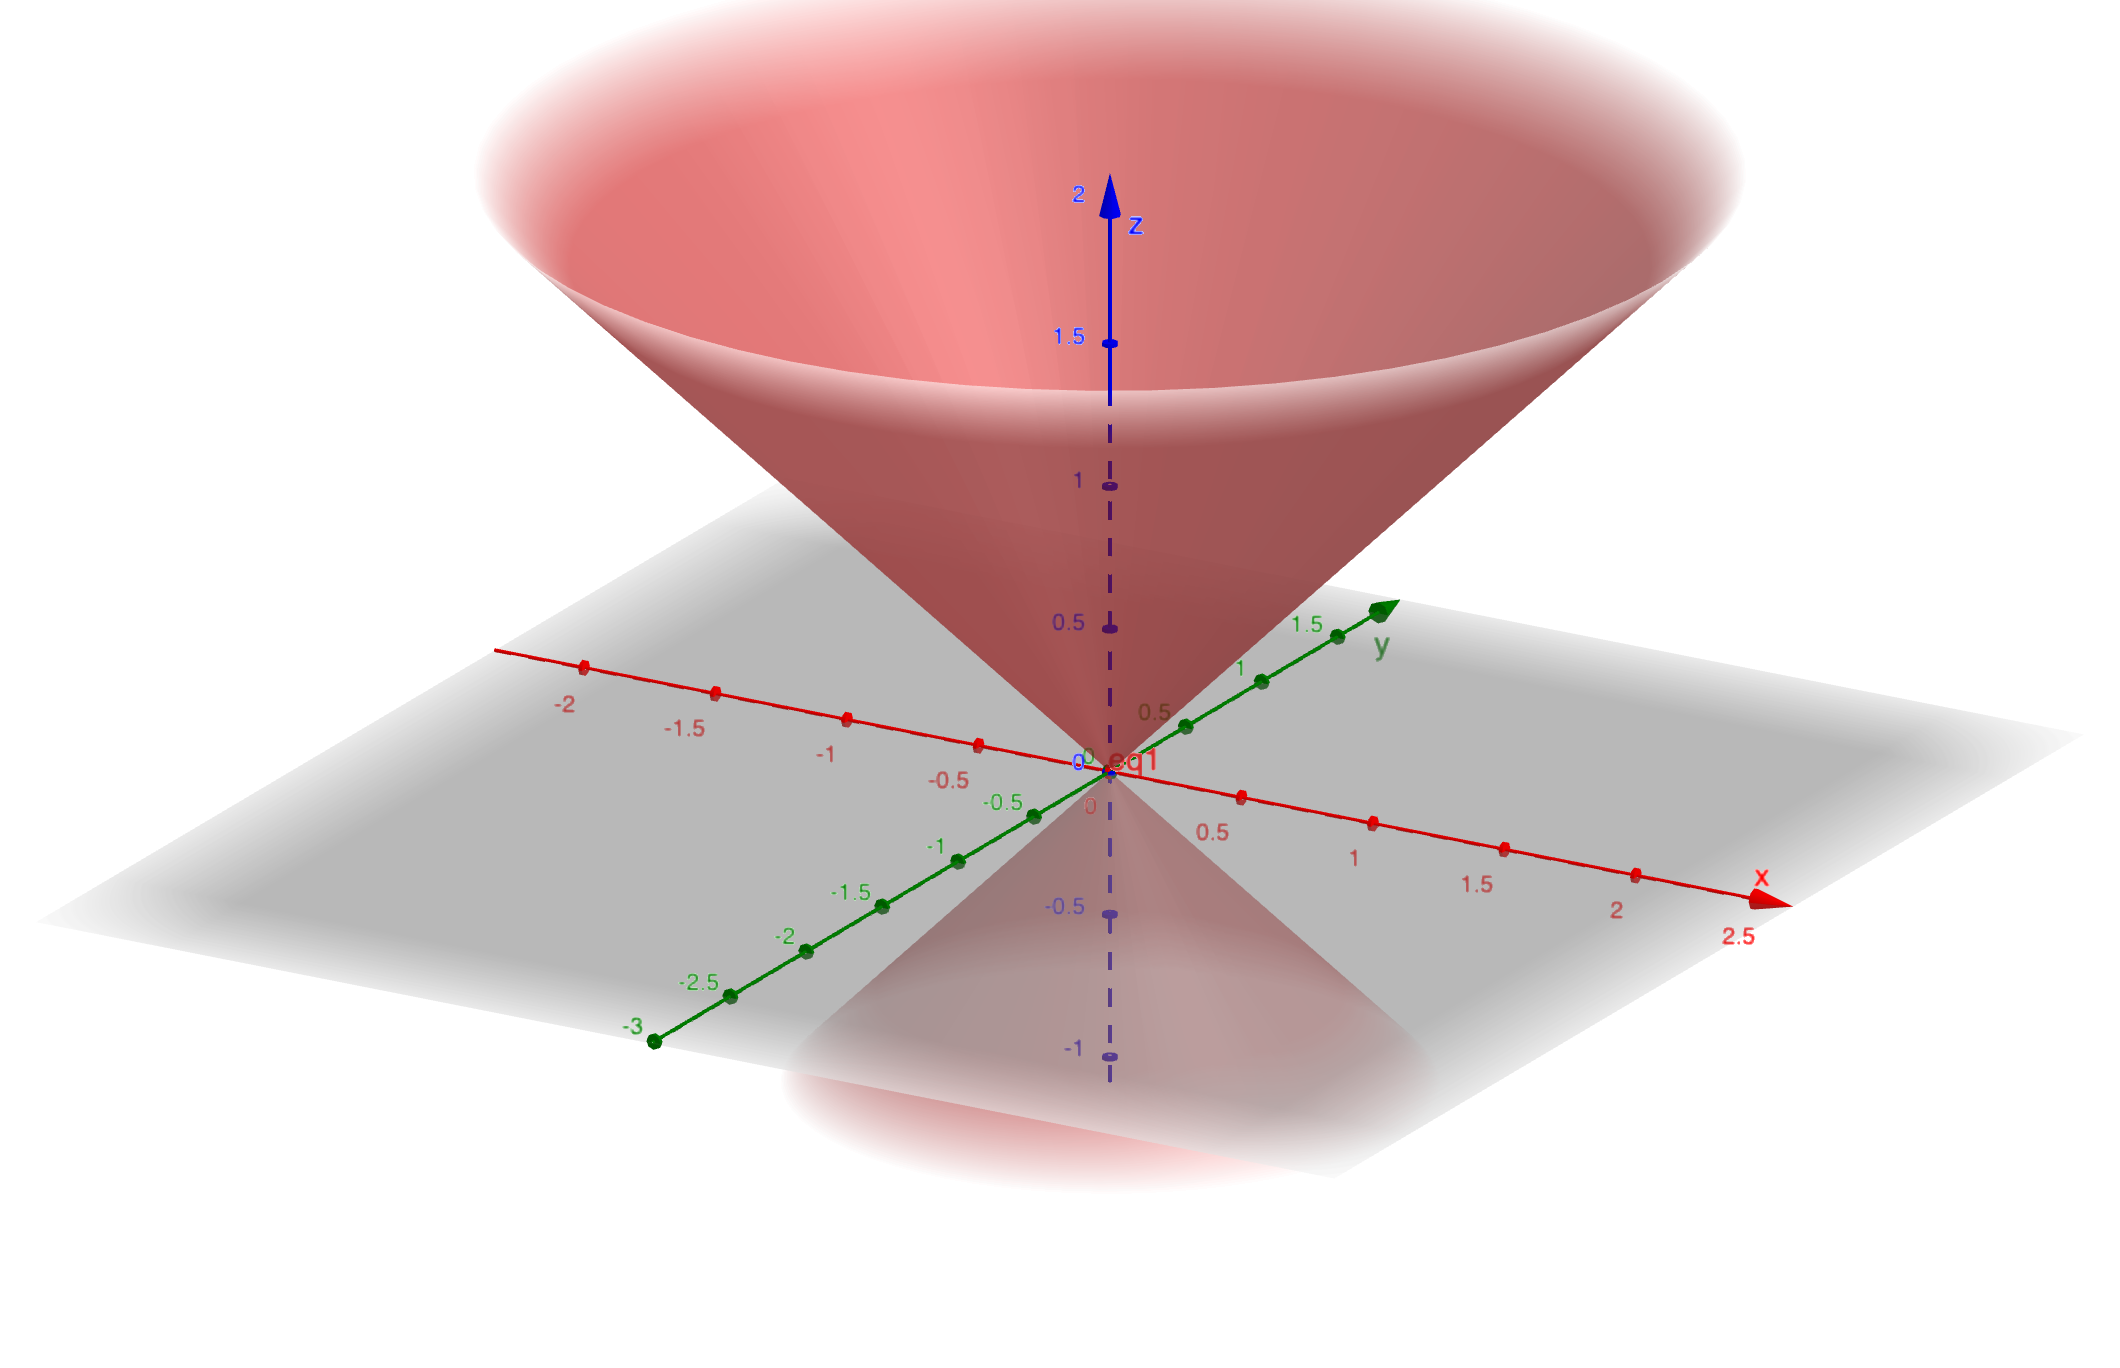
\includegraphics[width=.4\textwidth]{Figures/cone_surface.png}
            \end{figure}
            
            \item If we take $c=1$ and set
            \[
            x^2+y^2-z^2=1
            \]
            we get the \emph{hyperboloid of one sheet}.  This looks like
            \begin{figure}[H]
                \centering
                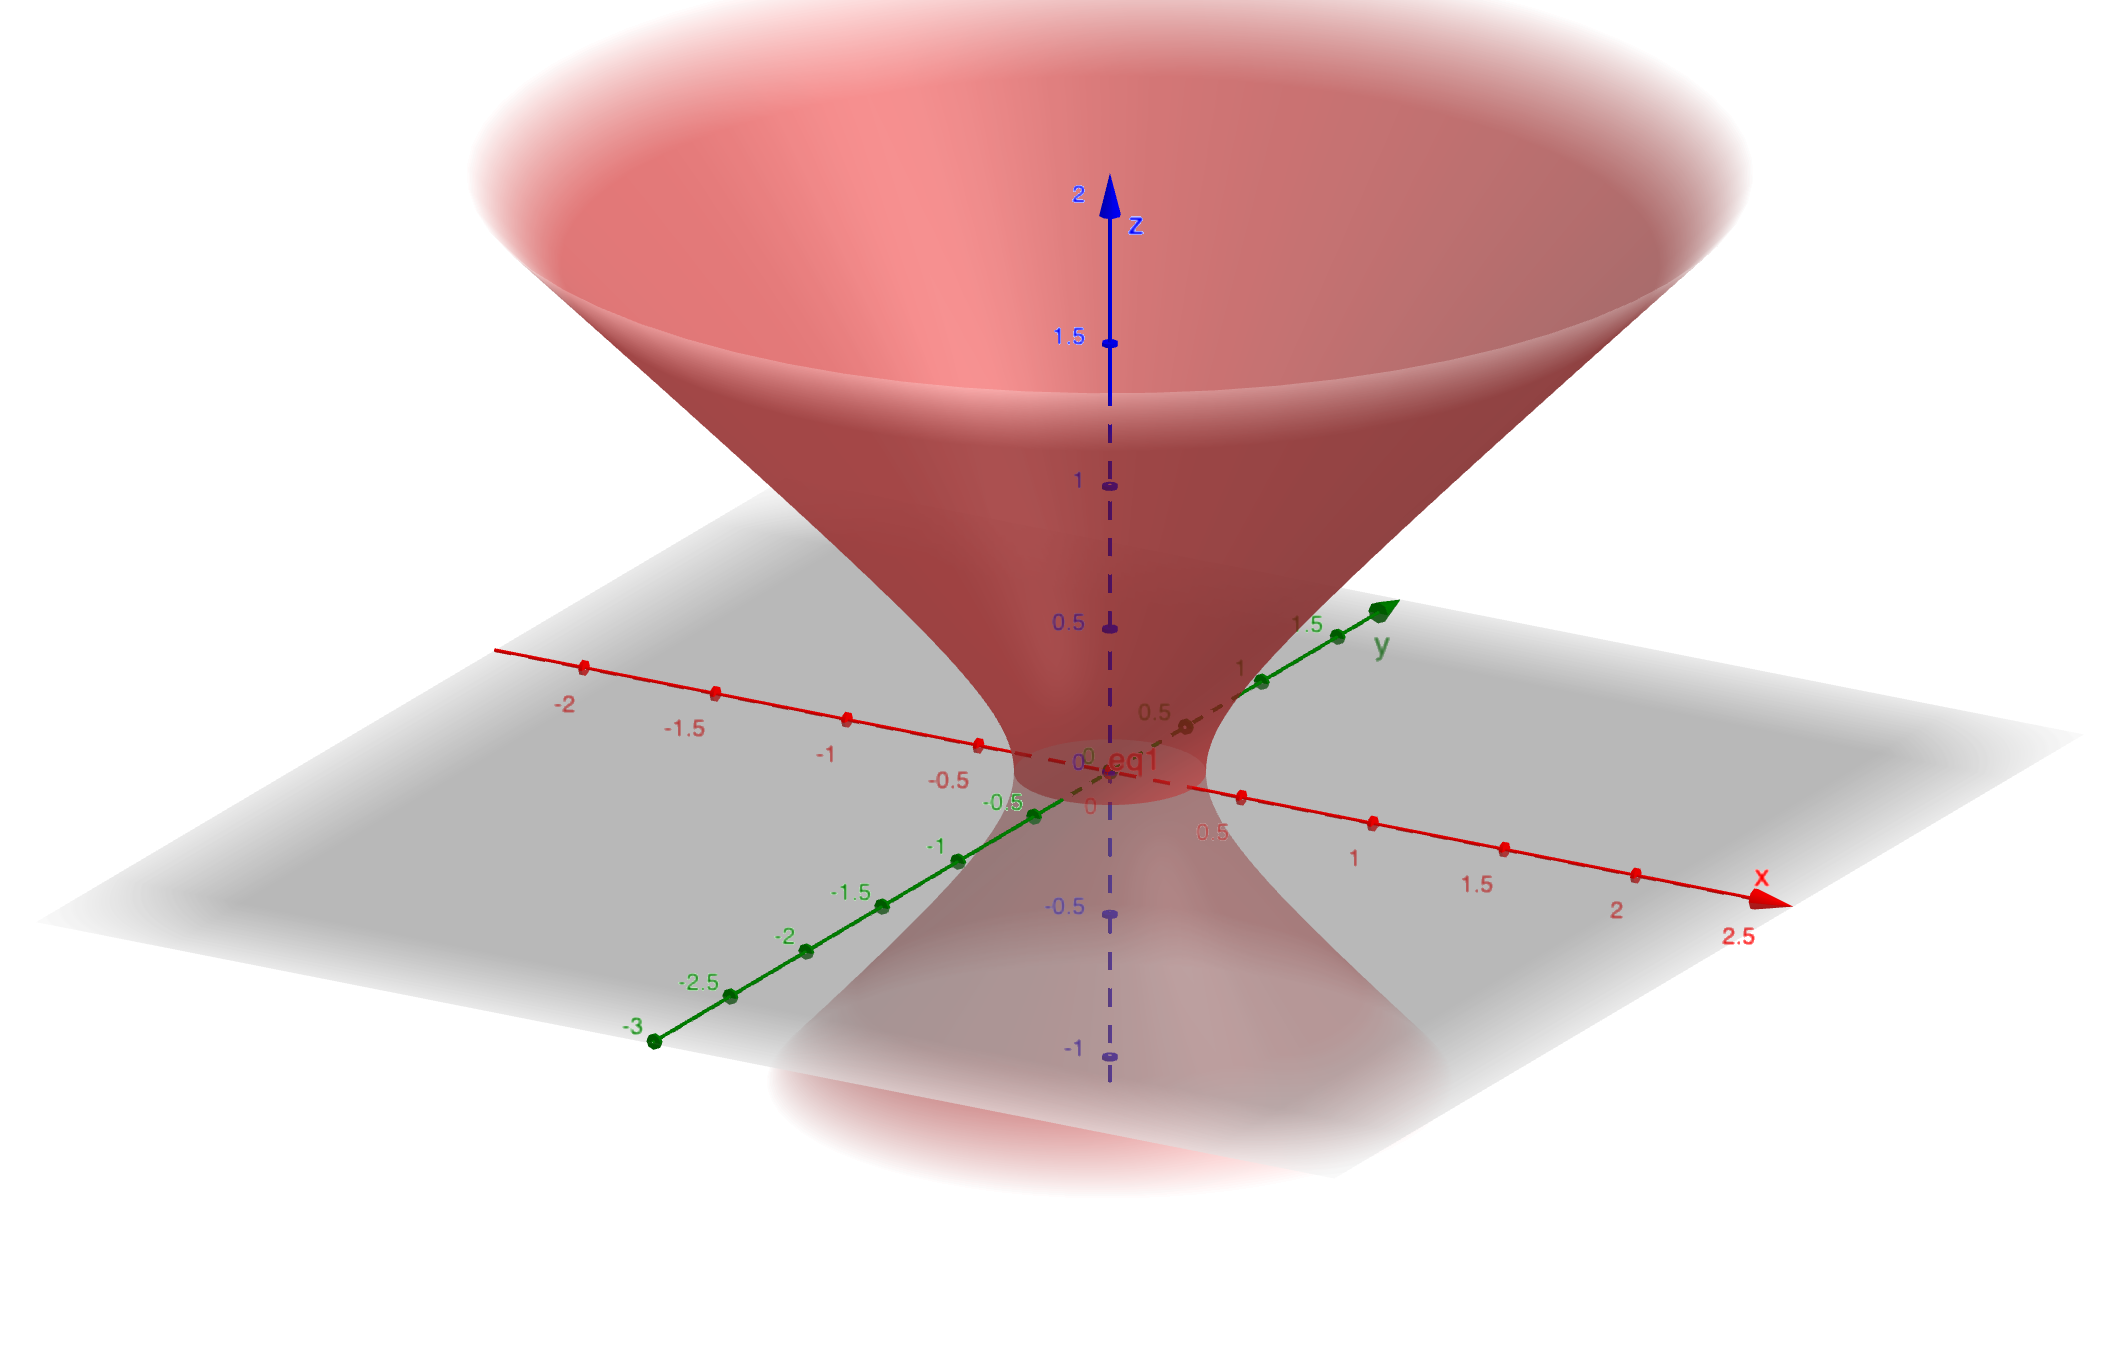
\includegraphics[width=.4\textwidth]{Figures/hyperboloid_1_sheet.png}
            \end{figure}
            
            \item If we take $c=-1$ and set
            \[
            x^2+y^2-z^2=-1
            \]
            we get the \emph{hyperboloid of two sheets}.  This looks like
            \begin{figure}[H]
                \centering
                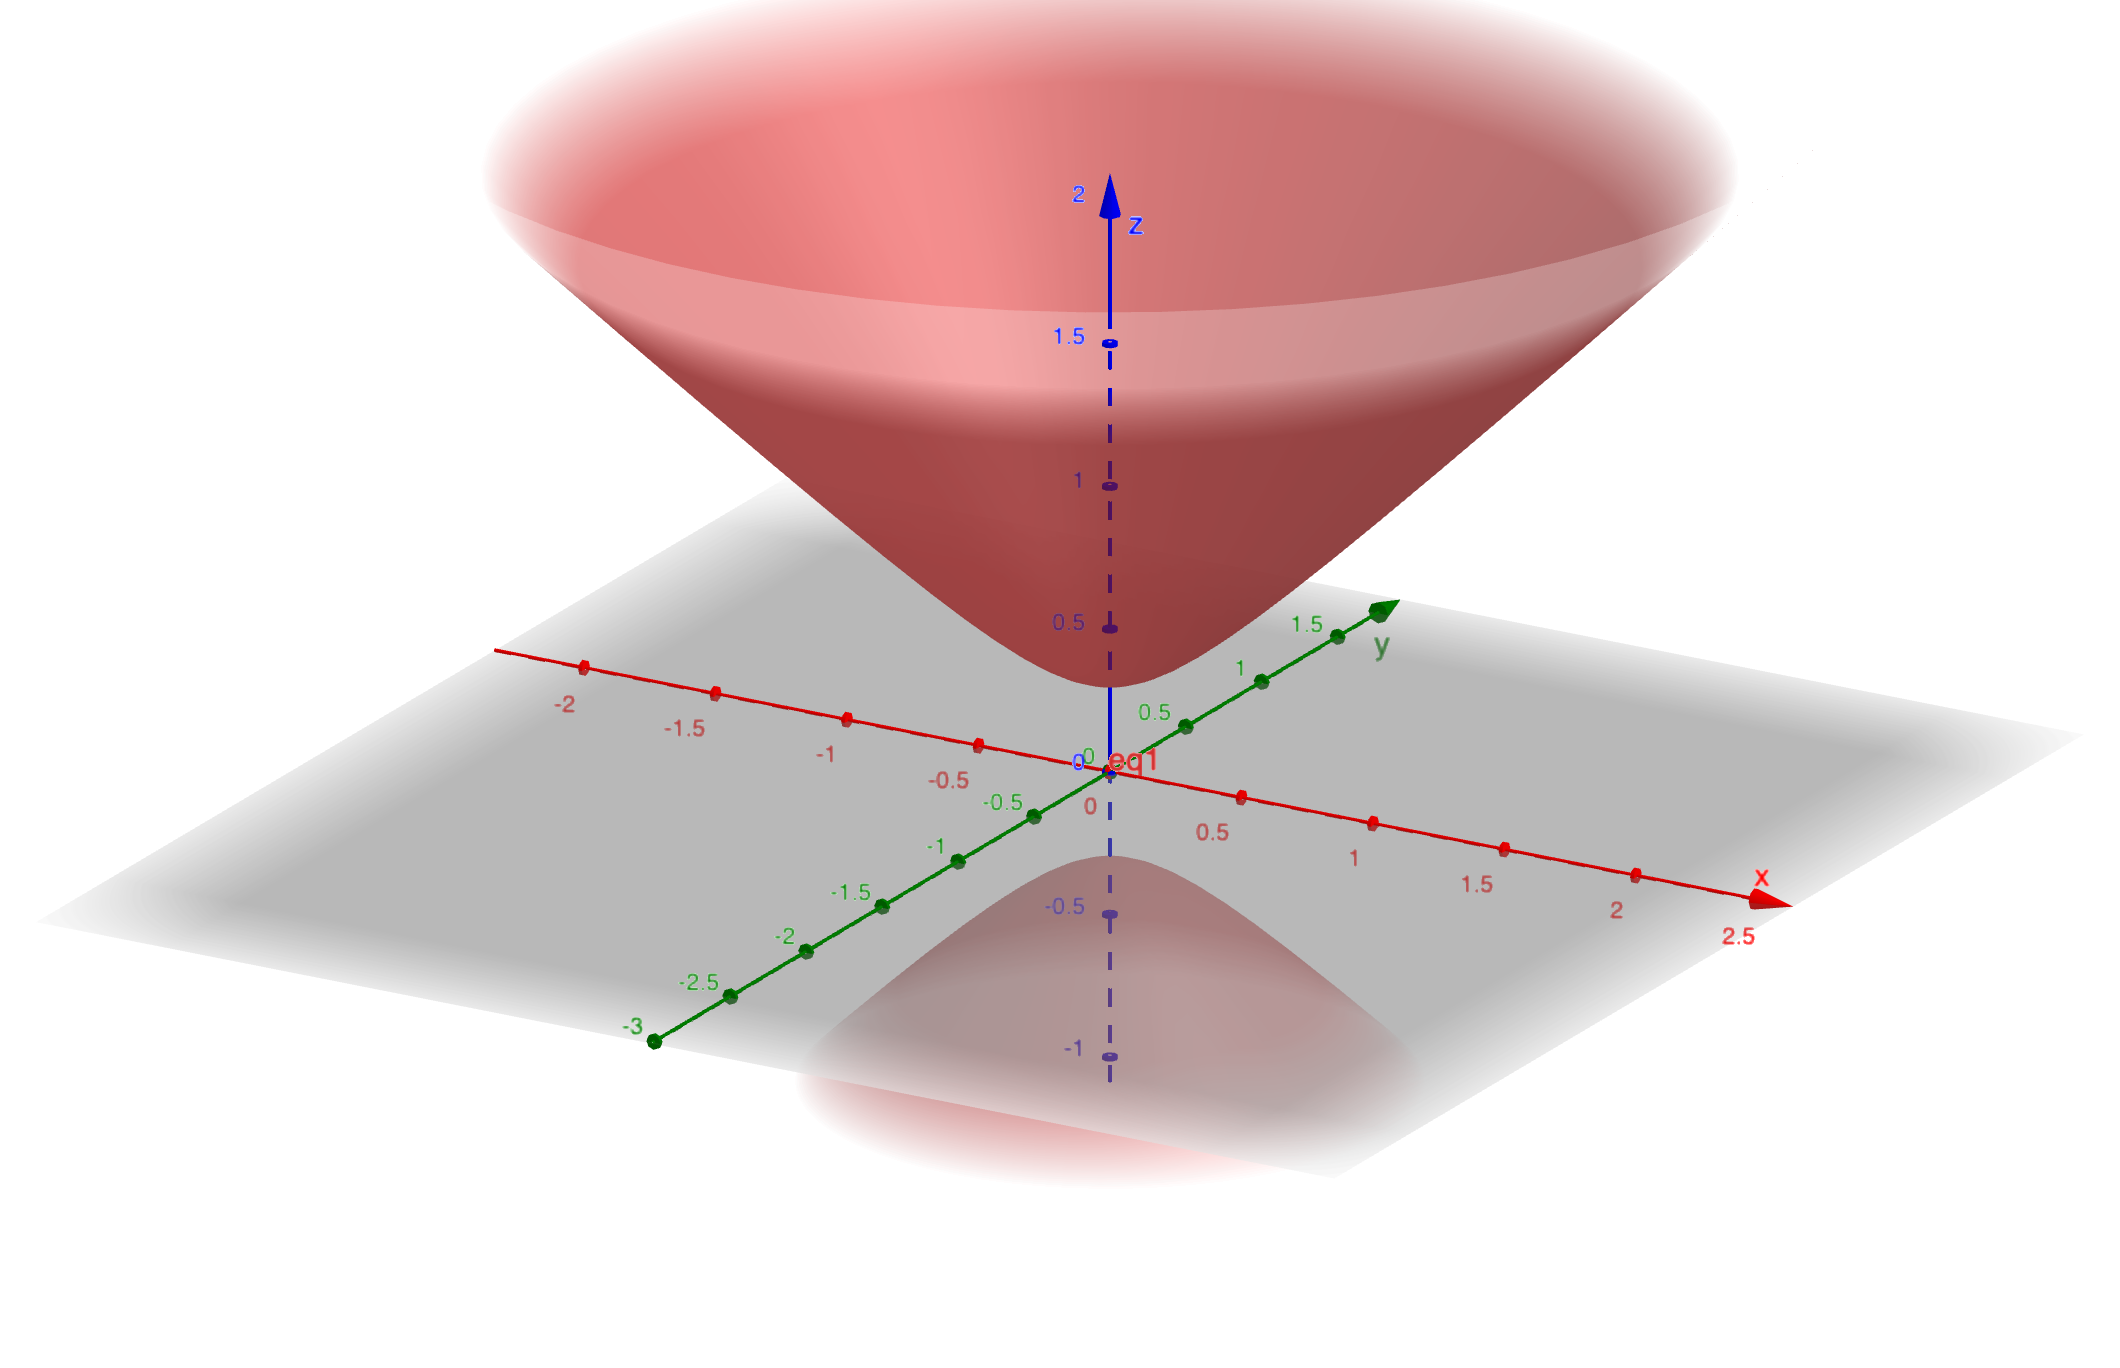
\includegraphics[width=.4\textwidth]{Figures/hyperboloid_2_sheet.png}
            \end{figure}
        \end{itemize}
        \end{ex}
        
        \begin{ex}{The Torus}{torus}
        For this example, I will choose specific nice numbers, but this is a yet another case of a level surface.  Take
        \[
        \left(5-\sqrt{x^2+y^2}\right)^2+z^2=2.
        \]
        This gives us the \emph{torus} with inner radius (the radius from the center of the donut hole to the center of the tube) $5=R$ and tube radius $2=r$. This looks like
        \begin{figure}[H]
            \centering
            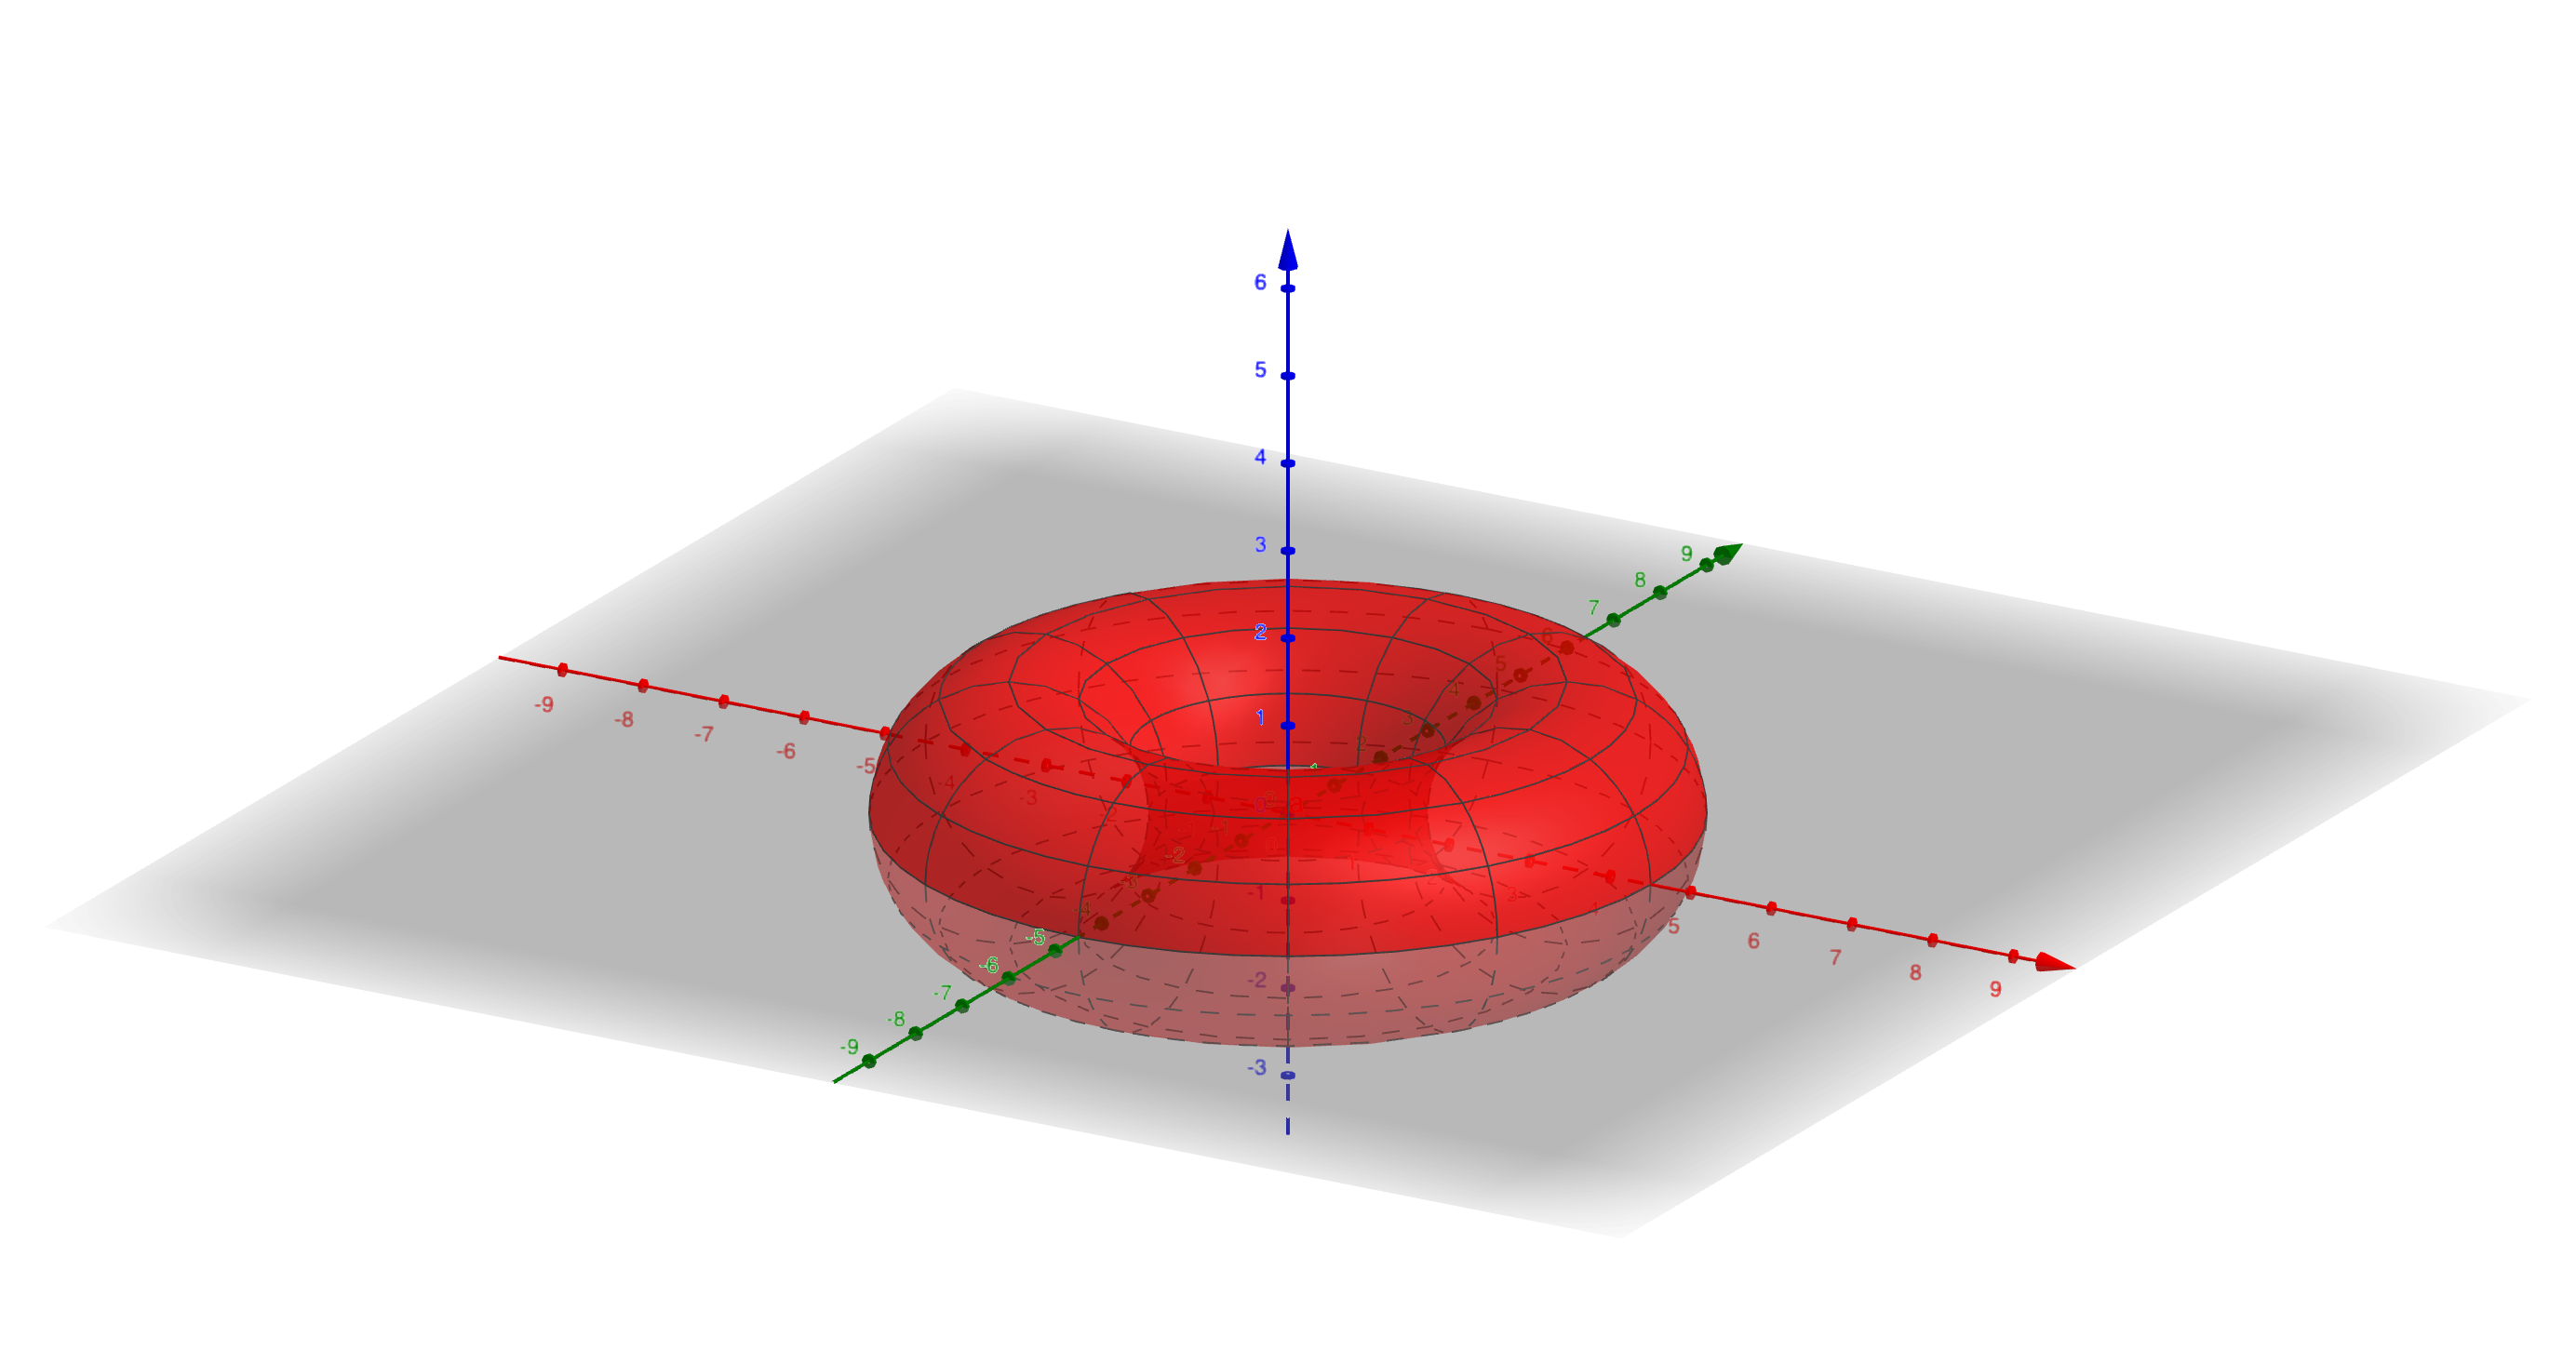
\includegraphics[width=.4\textwidth]{Figures/torus.png}
        \end{figure}
        \end{ex}
        
        
        We have given ourselves ways of understanding the scalar functions and curves, but still need to develop a manner to understand vector fields.  We will not only need to understand vector fields in their own right, but we will need them in order to investigate how the scalar fields change from point to point.  Roughly speaking, the ``derivative" of a scalar field will be a vector field.
        
        \section{Vector Fields}
        
        A vector field is a function that inputs a vector and outputs a vector. Specifically, we can write
        \[
        \mathbf{v}(x,y,z)=(f_1(x,y,z),f_2(x,y,z),f_3(x,y,z))=\begin{bmatrix} f_1(x,y,z)\\ f_2(x,y,z) \\ f_3(x,y,z)\end{bmatrix}.
        \]
        Notice the differences and similarities between vector fields, scalar fields, and curves.  Just as before, it will be nice to visualize many vector fields in the $xy$-plane to avoid drawing in 3-dimensions. Of course, we can use technology to make nice plots in space.
        
        Intuitively, a vector field is an assignment of a vector at each point in space.  To match this intuition we tend to just draw a collection of arrows in space.
        
        \begin{ex}{Eastward Wind}{east_wind}
        Consider the vector field
        \[
        \mathbf{v}\colon \R^2 \to \R^2
        \]
        given by
        \[
        \mathbf{v}(x,y)=(1,0).
        \]
        At each point $(x,y)$, we are assigning a vector that points a distance 1 in the $x$-direction. See the following figure.
        \begin{figure}[H]
            \centering
            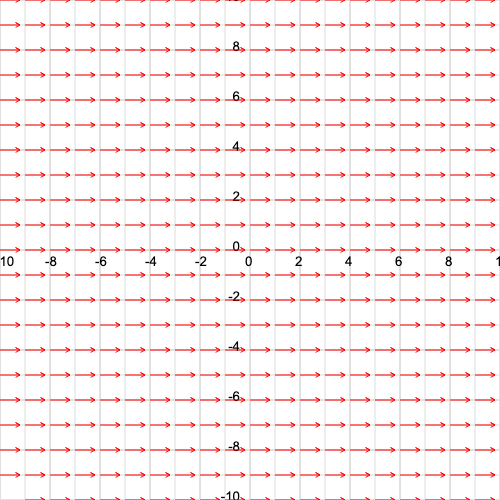
\includegraphics[width=.6\textwidth]{Figures/wind_field.png}
        \end{figure}
        \end{ex}
        
        \begin{ex}{Line Source}{line_source}
        Consider the vector field in the plane given by
        \[
        \mathbf{v}(x,y)=(x+y,x+y).
        \]
        See the following figure.
        \begin{figure}[H]
            \centering
            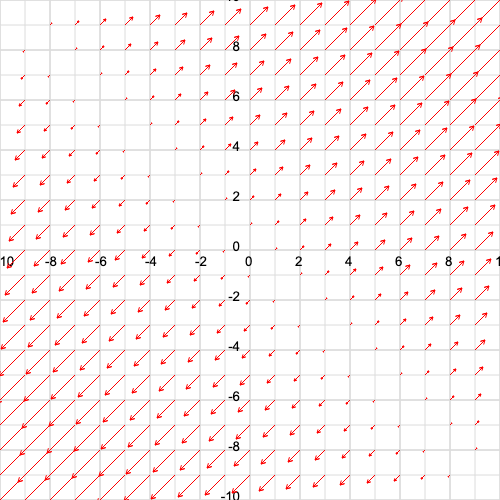
\includegraphics[width=.6\textwidth]{Figures/v_field_1.png}
        \end{figure}
        \end{ex}
        
        \begin{ex}{Whirlpool}{whirlpool}
        Consider the vector field in the plane given by
        \[
        \mathbf{v}(x,y)=(y,-x).
        \]
        See the following figure.
        \begin{figure}[H]
            \centering
            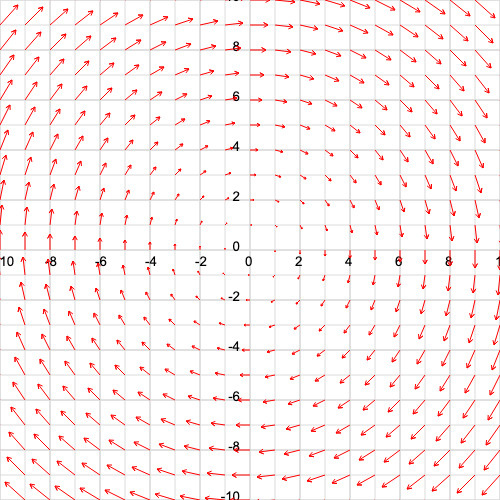
\includegraphics[width=.6\textwidth]{Figures/v_field_3.png}
        \end{figure}
        \end{ex}
        
    \chapter{Calculus with Multivariate Functions}
        
        \section{Differentiation of fields}
        One may now wonder where the calculus comes in.  We are almost there, but we should know what it means intuitively to use the calculus tools with these more general fields.
        
        Curves will prove to be a great tool in the analysis of these scalar fields.  We will also need to understand how vectors transform from point to point which will require us to recall the knowledge we gained on linear transformations.
        
        Roughly speaking, we will have:
        \begin{itemize}
            \item \textbf{Curves:} Derivatives of curves $\gamma(t)$ are vectors. Specifically, we have already seen the tangent vector $\gamma'(t)$ and acceleration vector $\gamma''(t)$.
            \item \textbf{Scalar Fields:} Derivatives of scalar fields $f(x,y,z)$ will depend on which input of the function we change.  We can collect the partial derivatives corresponding to finding derivatives in one input into a vector called the \emph{gradient}.
            \item \textbf{Vector Fields:} Derivatives of vector fields $\mathbf{v}(x,y,z)$ will require us to see how each component of $\mathbf{v}$ changes based on how each individual input changes.  In this case, this collection of derivatives will be put into a matrix known as the \emph{total derivative}.
        \end{itemize}
        
        \begin{remark}
        The important notion that we need to understand is the following.
        
        \emph{The derivative of a function at a point is the best linear approximation to the function.} 
        
        Based on this wording, it is intuitive to imagine derivatives as vectors or matrices.
        \end{remark}
        
        \section{Functions of Fields}
        In our world, we often care about combining different fields together.  For example, we can take the electric field created by a single charged particle and add this field to another field created by a different charged particle. What I mean, is we can write
        \[
        \mathbf{v}(x,y,z)+\mathbf{u}(x,y,z)
        \]
        and make sense of this.  Just as we did with vectors, we add the components together! That is if we have
        \begin{align*}
        \mathbf{v}(x,y,z)&=(f_1(x,y,z),f_2(x,y,z),f_3(x,y,z))\\ \mathbf{u}(x,y,z)&=(g_1(x,y,z),g_2(x,y,z),g_3(x,y,z)),
        \end{align*}
        then
        \[
        \mathbf{v}(x,y,z)+\mathbf{u}(x,y,z)=(f_1+g_1,f_2+g_2,f_3+g_3).
        \]
        Intuitively, this just adds together the vectors at each point!
        
        \begin{ex}{Addition of vector fields}{add_vect_fields}
        Consider the following vector fields
        \begin{align*}
            \mathbf{v}(x,y)&=(x,x)\\
            \mathbf{u}(x,y)&=(y,y).
        \end{align*}
        These look like:
        \begin{figure}[H]
            \centering
            \begin{subfigure}[h]{.45\textwidth}
            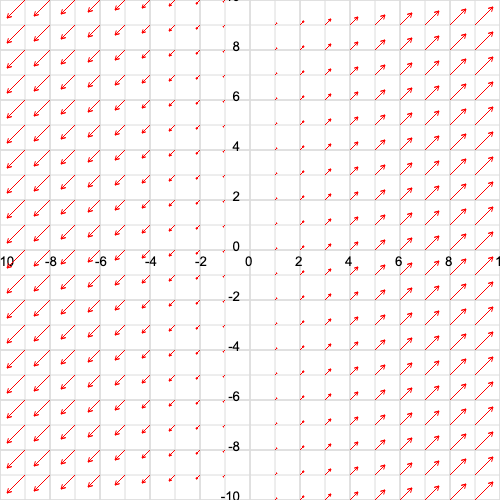
\includegraphics[width=\textwidth]{Figures/vec_v.png}
            \caption{Vector field $\mathbf{v}$.}
            \end{subfigure}
            ~
            \begin{subfigure}[h]{.45\textwidth}
            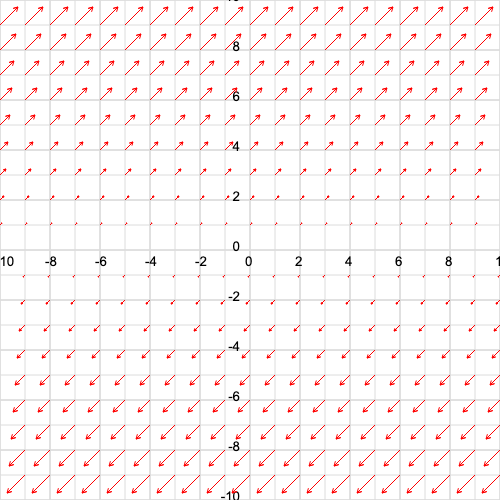
\includegraphics[width=\textwidth]{Figures/vec_u.png}
            \caption{Vector field $\mathbf{u}$.}
            \end{subfigure}
        \end{figure}
        Adding these results in the field
        \begin{figure}[H]
            \centering
            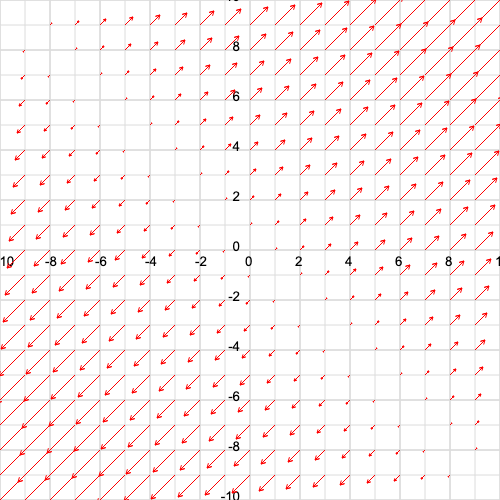
\includegraphics[width=.45\textwidth]{Figures/v_field_1.png}
            \caption{Caption}
            \label{fig:vec_field_1}
        \end{figure}
        \end{ex}
%        
        \begin{remark}
        If we do this all for vector fields, we can take curves and scalar fields as special cases.
        \begin{itemize}
            \item Adding together scalar fields is the same as adding functions.  They just have more inputs to think about!
            \item Adding together curves is done in the same componentwise manner that we have shown here for vector fields.
        \end{itemize}
        \end{remark}
        
        We can also scale a field by a real number.  This will stretch vectors at each point.
        
        \begin{ex}{Scaling of Vector Fields}{scale_vect_field}
        Just take the vector field
        \[
        \mathbf{v}(x,y,z)=(f_1(x,y,z),f_2(x,y,z),f_3(x,y,z))
        \]
        then we can take
        \[
        \lambda \mathbf{v}=(\lambda f_1, \lambda f_2, \lambda f_3).
        \]
        \end{ex}
        
        \begin{remark}
        There is many reasons why the above is important.  It seems our physical world plays nicely with the above concept, for one.
        
        One thing we can actually do, and will do a bit later, is find that there are two main types of vector fields in $\R^3$.  These will be the curl fields and divergence fields!  This is important in electromagnetism.
        \end{remark}
        
        When we were working with complex numbers, we considered integrating a complex function $f(z)$ over a contour $\gamma(t)$ from $t=a$ to $t=b$.  This involved computing
        \[
        \int_\gamma f(\gamma)d\gamma = \int_a^b f(\gamma(t))\gamma'(t)dt.
        \]
        I introduced this concept since it appears in the context of multivariate functions.  However, in the multivariate case, we needed some more tools.
        
        Now, the idea is as follows.  We will be given a scalar field, $f(x,y,z)$ or a vector field $\mathbf{F}(x,y,z)$ and a curve $\gamma(t)$.  
        
        \section{Line integrals of scalar fields}
        For the purpose of visualization, we will look at scalar fields of two variables and curves in the plane.  Our set up will have $f(x,y)$ and $\gamma(t)$ over the time $t=a$ to $t=b$.
        
        We want to understand the following:
        \[
        \int_\gamma f(\gamma)d\gamma \coloneqq \int_a^b f(\gamma(t))\|\gamma'(t)\|dt.
        \]
        Intuitively speaking, this integral finds the area under the curve $\gamma$ along the graph of $f$.  This is analogous to what we did in one dimension! See the following figure.
        \begin{figure}[H]
            \centering
            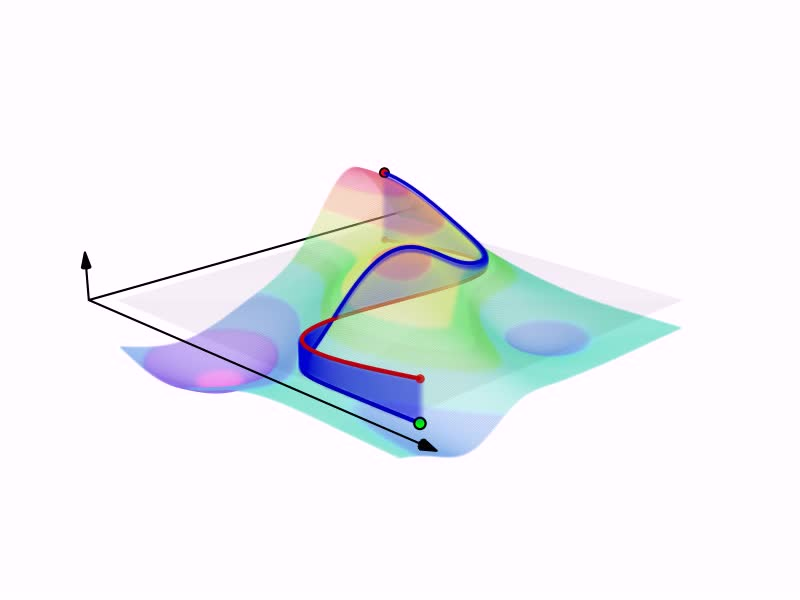
\includegraphics[width=.5\textwidth]{Figures/Line_integral_of_scalar_field.jpg}
        \end{figure}
        
        \begin{ex}{Length of a curve}{length_of_curve}
        Let $f(x,y,z)=1$ and $\gamma(t)$ be a curve over $t=a$ to $t=b$.  Then the line integral
        \[
        \int_\gamma f(\gamma)d\gamma = \int_a^b \|\gamma'(t)\|dt
        \]
        is known as the \emph{length} (sometimes \emph{arclength} of the curve $\gamma$.
        \end{ex}
        
        \begin{ex}{Line Integral on a Paraboloid}{line_int_parabooid}
        Consider the function $f(x,y)=x^2+y^2$ and $\gamma(t)=(t,t)$ over $t=0$ to $t=1$.  Then the line integral
        \[
        \int_\gamma f(\gamma)d\gamma = \int_0^1 f(\gamma(t))\|\gamma'(t)\|dt.
        \]
        We have
        \begin{itemize}
            \item $f(\gamma(t))=t^2+t^2=2t^2.$
            \item $\|\gamma'(t)\|=\|(1,1)\|=\sqrt{2}.$
        \end{itemize}
        So we have
        \[
        \int_\gamma f(\gamma)d\gamma = \int_0^1 2\sqrt{2}t^2dt.
        \]
        This evaluates to $\frac{2\sqrt{2}}{3}$.
        \end{ex}
        
        \begin{exercise}
        Integrate $f(x,y)=x+y$ along the curve $\gamma(t)=(t,0)$ from $t=0$ to $t=1$. What do you notice about this? Can we tie this to one-dimensional integration?
        \end{exercise}
        
        \section{Line integrals of vector fields}
        
        There is also a type of line integral that works alongside vector fields.  Roughly, the idea is to add up how much a vector field is pointing along the curve throughout the length of the curve.  
        
        Here we are given $\mathbf{F}(x,y,z)$ is a vector field, $\gamma(t)$ is a curve over the time $t=a$ to $t=b$.  Then we can write
        \[
        \int_\gamma \mathbf{F}(\gamma)\cdot d\gamma =\int_a^b \mathbf{F}(\gamma(t))\cdot \gamma'(t) dt.
        \]
        
        \begin{ex}{Work Done on a Particle}{work_on_particle}
        The work done on a particle (or change in energy) is written as a line integral of this form.  
        
        Take for example, $\mathbf{F}(x,y)=(2x,3y)$ and $\gamma(t)=(t,t^2)$ over the time $t=0$ to $t=1$.  Then
        \begin{align*}
        \int_\gamma \mathbf{F}(\gamma)\cdot d\gamma &= \int_0^1 \mathbf{F}(t,t^2)\cdot (t,t^2)dt\\
        &= \int_0^1 (2t,2t^2)\cdot(t,t^2)dt\\
        &=\int_0^1 2t^2+2t^4dt.
        \end{align*}
        Which I'll leave to you to evaluate if you'd like.
        \end{ex}
        
        \begin{remark}
        This notion is extremely important in defining something called the \emph{potential} of a vector field.  This will show up in electrodynamics.
        
        If the force in the example above is \emph{conservative}, we will have a potential.  This will correspond nicely to the vector field having no \emph{curl}.
        \end{remark}
        
        \section{Derivatives}
        Having done some integral calculus, it's time to head back to differential calculus.  We should say the following. This is far more abstract than we need, but it is an important realization.  
        
        \begin{df}{The Derivative}{derivative}
        Given a function $f\colon \R^n \to \R^m$, the \textbf{derivative of $f$ at the point $\mathbf{x}_0$} is the best \emph{linear approximation} to $f$ at the point $\mathbf{x}_0$.
        
        What this means is the following: If we zoom in to the point $\mathbf{x}_0$ and see what $f$ does in this region, we'll notice that $f$ is approximately a linear transformation.
        \end{df}
        
        Now, let us review the one-dimensional derivative that we are familiar with.
        
        \begin{df}{Derivative on $\R$}{der_on_R}
        Given $f\colon \R \to \R$, we define the \textbf{derivative $f'$ of $f$ at the point $x_0$} by
        \[
        f'(x_0)\coloneqq \lim_{\delta \to 0} \frac{f(x_0+\delta)-f(x_0)}{\delta}.
        \]
        This value $f'(x_0)$ is a number, and moreover is a $1\times 1$-matrix!  We often hide this idea at first.
        \end{df}
        
        It's a bit silly to say $f'(x_0)$ is a $1\times 1$-matrix, but in the end it will help us to remember this.
        
        \subsubsection{Derivatives of scalar fields}
        We can investigate functions of multiple variables in more ways than the single variable case.  Let us start with scalar fields.
        
        \begin{df}{Partial Derivatives}{partial_derivs}
        Let $f\colon \R^3 \to \R$ be a scalar field.  Then we can consider derivatives with respect to changing each input.  For example, we define the \textbf{partial derivative with respect to $x$} \textbf{at the point $(x_0,y_0,z_0)$}, denoted $\frac{\partial f}{\partial x}$, and put
        \[
        \frac{\partial f}{\partial x}(x_0,y_0,z_0)\coloneqq \lim_{\delta \to 0} \frac{f(x_0+\delta,y_0,z_0)-f(x_0,y_0,z_0)}{\delta}
        \]
        \end{df}
        
        \begin{remark}
        For partial derivatives, all but one variable are being held constant.  So, when you are computing these, be sure to treat the proper variables as constant when necessary.
        \end{remark}
        
        \begin{exercise}
        Define $\frac{\partial f}{\partial y}$ and $\frac{\partial f}{\partial z}$ in a similar way to the above definition.
        \end{exercise}
        
        \begin{exercise}
        Compute $\partialx$, $\partialy$, and $\partialz$ for the function 
        \[
        f(x,y,z)=\sin(xyz)+x+2y^2+3x^2z.
        \]
        \end{exercise}
        
        It turns out that collecting the partial derivatives as a vector is the best linear approximation to a scalar function.  We call this vector the gradient vector.
        
        \begin{df}{The Gradient}{gradient}
        Given a scalar field $f(x,y,z)$, the \textbf{gradient of $f$ at the point $(x_0,y_0,z_0)$}, denoted $\nabla f(x_0,y_0,z_0)$ is given by
        \[
        \nabla f(x_0,y_0,z_0)=\begin{bmatrix} \partialx(x_0,y_0,z_0)\\ \partialy(x_0,y_0,z_0)\\ \partialz(x_0,y_0,z_0)\end{bmatrix}.
        \]
        \end{df}
        
        \begin{exercise}
        Compute the gradient for the function
        \[
        f(x,y,z)=\sin(xyz)+x+2y^2+3x^2z.
        \]
        \end{exercise}
        
        \subsubsection{Properties of partial derivatives and the gradient}
        
        As with the one-dimensional derivative, we have some properties that will be helpful.\\
        
        \noindent\textbf{Partial Derivatives:}
        \begin{enumerate}[(i)]
            \item \textbf{Sum Rule:} Given $f(x,y,z)$ and $g(x,y,z)$, we have that
            \[
            \frac{\partial}{\partial x} (f(x,y,z)+g(x,y,z))=\partialx + \frac{\partial g}{\partial x}.
            \]
            Of course, this holds for any partial derivative.
            \item \textbf{Constant Multiple:} Given $\lambda \in \R$ and $f(x,y,z)$, we have that
            \[
            \frac{\partial}{\partial x}(\lambda f(x,y,z))=\lambda \partialx.
            \]
            Again, this holds for any partial derivative.
            \item \textbf{Product Rule:} Given $f(x,y,z)$ and $g(x,y,z)$ we have that
            \[
            \frac{\partial }{\partial x}(f(x,y,z)g(x,y,z))=\partialx g + f \frac{\partial g}{\partial x}.
            \]
            Ths holds for all partial derivatives.
        \end{enumerate}
        
        \begin{remark}
        The chain rule will show up eventually, but not yet.  As for the quotient rule, this also holds, but I don't show it here.
        \end{remark}
        
        \noindent\textbf{The Gradient:}
        \begin{enumerate}[(i)]
            \item \textbf{Sum Rule:} Given $f(x,y,z)$ and $g(x,y,z)$, we have that
            \[
            \nabla(f(x,y,z)+g(x,y,z))=\nabla f(x,y,z)+\nabla g(x,y,z).
            \]
            \item \textbf{Constant Multiple:} Given $\lambda \in \R$ and $f(x,y,z)$, we have that
            \[
            \nabla(\lambda f(x,y,z))=\lambda \nabla f(x,y,z).
            \]
            \item \textbf{Product Rule:} Given $f(x,y,z)$ and $g(x,y,z)$ we have that
            \[
            \nabla(f(x,y,z)g(x,y,z))=(\nabla f(x,y,z))g(x,y,z)+f(x,y,z)(\nabla g(x,y,z))
            \]
            
        \end{enumerate}
        
        We've learned how to compute partial derivatives and the gradient, but what are they really telling us? Remember that the derivative $\frac{d}{dx}$ of a function $f(x)$ tells us the rate of change of $f$ as we move in the $x$-direction.  This is very similar to what $\frac{\partial}{\partial x}$ tells us about a function $f(x,y,z)$.  So we can say the following.
        \begin{itemize}
            \item $\frac{\partial f}{\partial x}$ tells us how $f$ changes as we move in the $x$-direction.
            \item $\frac{\partial f}{\partial y}$ tells us how $f$ changes as we move in the $y$-direction.
            \item $\frac{\partial f}{\partial z}$ tells us how $f$ changes as we move in the $z$-direction.
        \end{itemize}
        
        We can put these together into the gradient $\nabla f$ and know how $f$ changes in each possible direction. Let's see how the gradient acts then. 
        
        \begin{ex}{Gradients on the Paraboloid}
        Let us start with $f(x,y)=x^2+y^2$.  Then
        \[
        \nabla f(x,y) = (2x,2y).
        \]
        Let us plot the level curves of this surface.
        \begin{figure}[H]
            \centering
            \begin{subfigure}[h]{.45\textwidth}
            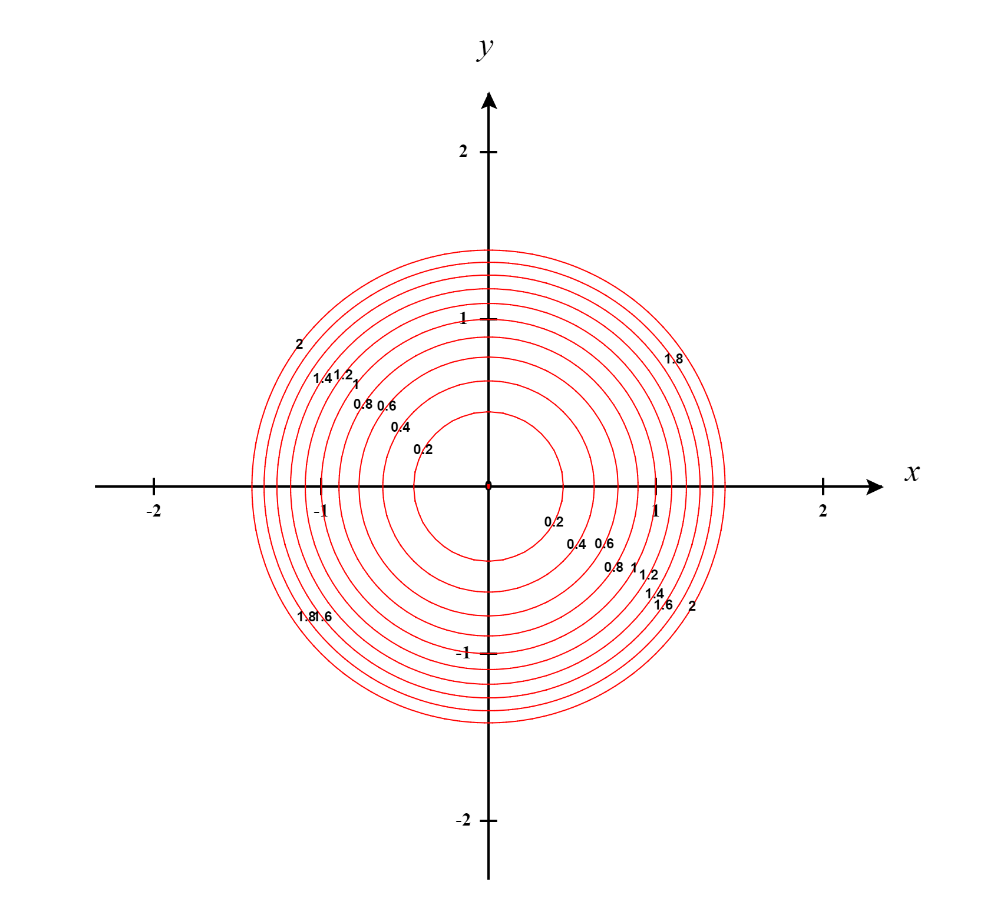
\includegraphics[width=\textwidth]{Figures/level_curves_gradient.png}
            \caption{Level curves of $f(x,y)$.}
            \end{subfigure}
            ~
            \begin{subfigure}[h]{.45\textwidth}
            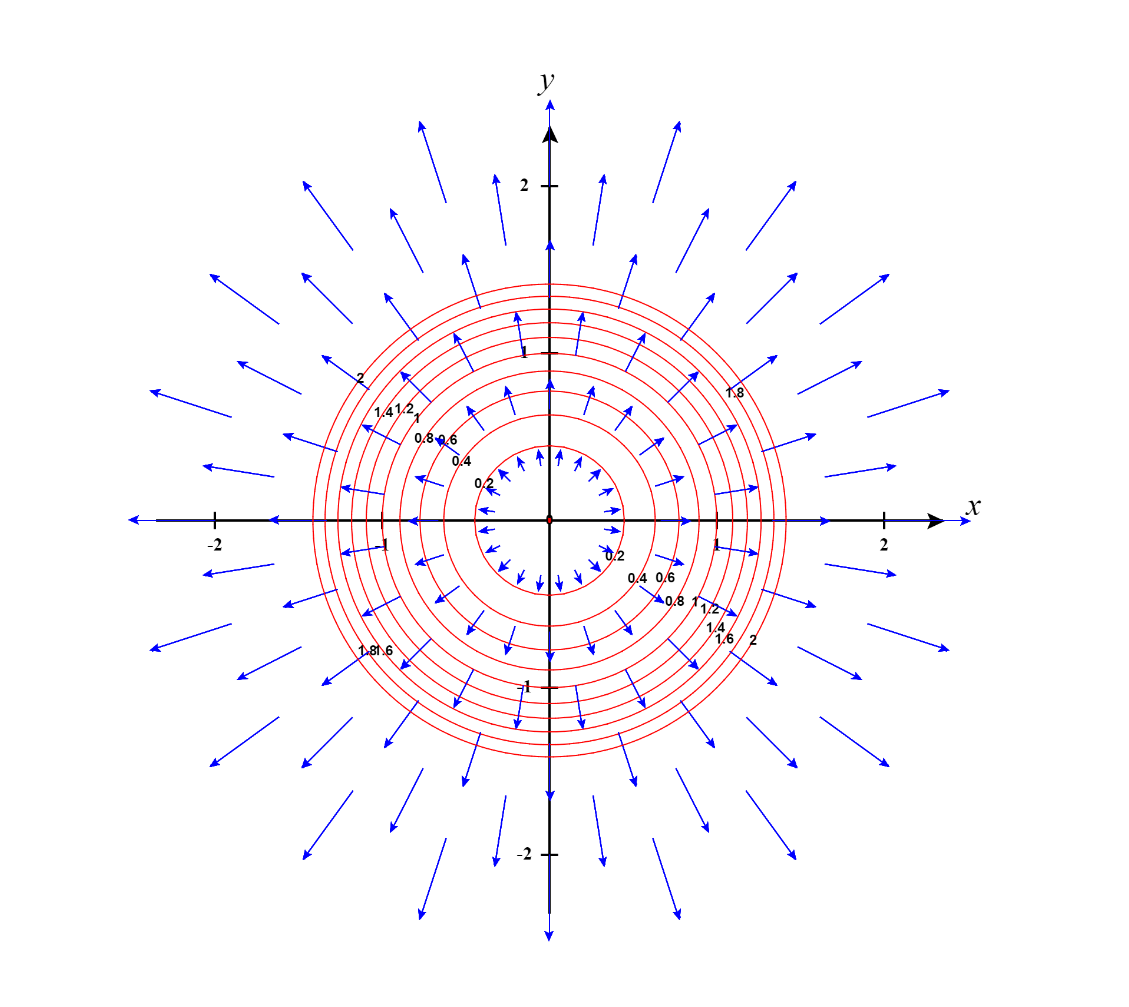
\includegraphics[width=\textwidth]{Figures/level_curves_gradient_vectors.png}
            \caption{Gradient vectors shown in blue.}
            \end{subfigure}
        \end{figure}
        \begin{itemize}
            \item Notice that the gradient vectors point in a direction perpendicular to the level curves and the length corresponds to how close the nearest level curve is.
            \item The gradient is zero at the bottom of this surface.  
        \end{itemize}
        \end{ex}
        
        \begin{prop}{Gradient Points Uphill}{gradient_prop}
        The gradient $\nabla f(x,y,z)$ is the vector that points in the direction of greatest increase for a function $f(x,y,z)$.
        \end{prop}
        
        How about second partial derivatives? What can we say here. We have each of the following for a function $f(x,y)$:
        \begin{itemize}
            \item $\frac{\partial^2 f}{\partial x^2}$
            \item $\frac{\partial^2 f}{\partial y^2}$
            \item $\frac{\partial}{\partial y}\frac{\partial f}{\partial x}$
            \item $\frac{\partial}{\partial x}\frac{\partial f}{\partial y}$
        \end{itemize}
        
        Recall what $\frac{d^2 f}{dx^2}$ meant for a function $f(x)$.  This told us how $f$ was curving (or what concavity $f$ had). The story is similar for these partial derivatives.
        
        \begin{itemize}
            \item $\frac{\partial^2 f}{\partial x^2}$ tells us about the concavity (or curvature) of $f$ as we move in the $x$ direction.
            \item $\frac{\partial^2 f}{\partial y^2}$ tells us about the concavity (or curvature) of $f$ as we move in the $y$ direction.
            \item We actually have that $\frac{\partial}{\partial y}\frac{\partial f}{\partial x}=\frac{\partial}{\partial x}\frac{\partial f}{\partial y}$.  This interpretation is a bit hard to deal with.  Let's not worry too much about it.
        \end{itemize}
        
        \begin{prop}{Partial Derivatives Commute}{partials_commute}
        We have that
        \[
        \frac{\partial}{\partial y}\frac{\partial f}{\partial x}=\frac{\partial}{\partial x}\frac{\partial f}{\partial y}.
        \]
        Moreover, for functions of more variables, we can say that the order we take derivatives does not matter.
        \end{prop}
        
        \begin{exercise}
        Given $f(x,y)=x^2+y^2$, compute
        \[
        \frac{\partial^2 f}{\partial x^2}, ~ \frac{\partial^2 f}{\partial y^2}, ~ \frac{\partial}{\partial y}\frac{\partial f}{\partial x},~ \frac{\partial}{\partial x}\frac{\partial f}{\partial y}.
        \]
        What can we say about the curvature of $f$ in the two directions? Does this make sense?
        \end{exercise}
        
        \section{Optimization}
        In single variable calculus, we optimized functions $f(x)$ by finding the point $x_0$ where 
        \[
        f'(x_0)=0.
        \]
        We called this a \emph{critical point}. We found if this optimizer $x_0$ was a maximizer or minimizer by checking the sign of second derivative $f''(x_0)$. We had
        \begin{align*}
            \textrm{Maximum: }& f''(x_0)<0\\
            \textrm{Minimum: }& f''(x_0)>0.
        \end{align*}
        
        In higher dimensions, this idea works similarly. We just have more to check. 
        
        \begin{df}{Stationary Points}{stationary_points}
        Given a function $f(x,y)$, we call a point $(x_0,y_0)$ a \textbf{stationary point} if 
        \[
        \nabla f(x_0,y_0) = \mathbf{0}.
        \]
        \end{df}
        
        As before, we will use second derivatives to find out whether this is a maximum or a minimum.
        
        \begin{prop}{Maximizers and Minimizers}{max_min}
        A stationary point $(x_0,y_0)$ is a 
        \begin{align*}
            \textrm{Maximizer if~ }& \frac{\partial^2 f}{\partial x^2} <0 \textrm{ ~and~ } \frac{\partial^2 f}{\partial y^2}<0,\\
            \textrm{Minimizer if~ }& \frac{\partial^2 f}{\partial x^2} >0 \textrm{ ~and~ } \frac{\partial^2 f}{\partial y^2}>0,\\
            \textrm{Saddle if otherwise.}
        \end{align*}
        \end{prop}
        
        \begin{exercise}
        Let
        \[
        f(x,y) = \frac{xy}{e^{x^2+y^2}}.
        \]
        \begin{enumerate}[(a)]
            \item Find all stationary points for $f$.
            \item Determine whether these points are minimizers or maximizers.
        \end{enumerate}
        \end{exercise}
        
        \begin{exercise}
        Show that $f(x,y)=xy$ has a saddle point at $(0,0)$.
        \end{exercise}
        
        \subsubsection{Lagrange Multipliers}
        Often times we are given a situation that we wish to find an optimum solution to, but we are somehow constrained.  A biological example would be fixing a given volume for a red blood cell, and finding the optimum shape so that oxygen diffusion is maximized.  A physical example would be finding the fastest path between two points when moving through a medium with varying viscosity.
        
        The idea is relatively tame. We are given the function to optimize
        \[
        f(x,y,z)
        \]
        and the constraining function
        \[
        g(x,y,z)=k.
        \]
        Then we must solve the equation
        \[
        \nabla f(x,y,z) = \lambda \nabla g (x,y,z)
        \]
        where $\lambda$ is called the \textbf{Lagrange multiplier}. Let's work through an example of solving this.
        
        \begin{ex}{Largest Box}{largest_box}
        Let's find the dimensions of the box with the largest volume if the total surface area is $64 cm^2$.  We must determine our function to optimize, which is the volume function
        \[
        V(x,y,z) = xyz.
        \]
        Our constraint is the surface area function $A(x,y,z)$ must be
        \[
        g(x,y,z)=2xy+2xz+2yz=64,
        \]
        which we will simplify as
        \[
        xy+xz+yz = 32.
        \]
        \begin{enumerate}
            \item We first take
            \[
            \nabla f(x,y,z) = \begin{bmatrix} yz \\ xz \\ xy \end{bmatrix}
            \]
            and
            \[
            \nabla g(x,y,z) = \begin{bmatrix} 2y+2z \\ 2x+2z \\ 2x+2y\end{bmatrix}.
            \]
            \item This gives us four equations to solve. Three are from the equation $\nabla f(x,y,z) =\nabla g(x,y,z)$
            \begin{align}
                yz &= \lambda (y+z)\\
                xz &= \lambda (x+z)\\
                xy &= \lambda (x+y),
            \end{align}
            and one is from the constraint $g(x,y,z)=64$
            \[
            xy+xz+yz = 32.
            \]
            \item Working through solving these can be nontrivial.  In this case, we can do the following: Multiply (1) by $x$, (2) by $y$, and $(3)$ by $z$.  Which gives us
            \begin{align*}
                xyz &= \lambda x(y+z)\\
                xyz &= \lambda y(x+z)\\
                xyz &= \lambda z(x+y)
            \end{align*}
            Now we can set the first two equal to find
            \[
            \lambda x(y+z)=\lambda y(x+z)
            \]
            which simplifies to 
            \[
            \lambda (xz-yz)=0
            \]
            meaning that $\lambda =0$ or $xz=yz$. Note that $\lambda =0$ is not possible since that will end up giving us zero surface area and we won't satisfy the constraint.
            
            Now $xz-yz=0$ means that $x=y$, which we can substitute back into the equations later. 
            
            We can set the last two equal to find
            \[
            \lambda y (x+z)=\lambda z(x+y)
            \]
            which with similar work tells us $z=y$.  So now we make note of $x=y$ and we have $x=y=z$.  
            
            So now we use the constraint equation with $x=y=z$ and find that we have
            \[
            x^2+y^2+z^2 = 3x^2 = 32
            \]
            which means that $x\approx 3.266$.  Thus
            \[
            V(3.266,3.266,3.266)\approx 34.8376
            \]
            is the largest volume.  \emph{This means our ideal solution is a cube!} 
            
        \end{enumerate}
        \end{ex}
        
        \section{Approximation and the Tangent Space}
        Sometimes it is helpful to know what a surface looks like up close.  In this case, the surface is best approximated by a plane.  This is analogous to how you can approximate functions of a single variable by a line.
        
        \begin{exercise}
        Compute the tangent line to $f(x)=2x^2+5$ at the point $x_0=3$.
        \end{exercise}
        
        \subsubsection{Equation for a Plane}
        
        We haven't worked much with planes in space yet, but we have seen surfaces.  In some sense, planes are the easiest surfaces.  They are, after all, linear objects.
        
        \begin{ex}{Plane and Normal}{plane_normal}
        The equation for a plane is given by
        \[
        ax+by+cz+ d = 0.
        \]
        Notice that this is a linear equation.
        
        Then the \emph{normal vector} to the plane is given by 
        \[
        \mathbf{n} = \begin{bmatrix} a \\ b \\ c\end{bmatrix}.
        \]
        We can see a diagram of this here.
        \begin{figure}[H]
            \centering
            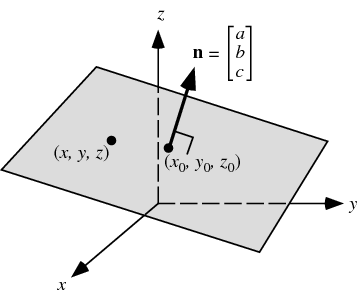
\includegraphics[width=.4\textwidth]{Figures/plane_n.png}
        \end{figure}
        \end{ex}
        
        Now, if we are given a surface (defined as a level surface or as the graph of a function), we can compute an approximation at a point called the \emph{tangent plane}.
        
        \begin{ex}{Tangent Plane to Paraboloid}
        Consider the function 
        \[
        f(x,y)=-x^2-y^2.
        \]
        Then the graph of the function is given by plotting the points
        \[
        (x,y,f(x,y)).
        \]
        We compute the tangent plane by computing partial derivatives. We take
        \begin{align*}
        \frac{\partial f}{\partial x} &= -2x\\    
        \frac{\partial f}{\partial y} &= -2y.
        \end{align*}
        Then the equation for a tangent plane at the point $(x_0,y_0,f(x_0,y_0))$ is given by
        \[
        z-f(x_0,y_0)=\partialx (x-x_0)+\partialy (y-y_0).
        \]
        So in our case, we have
        \[
        z-(-x_0^2-y_0^2)=-2x_0(x-x_0)-2y_0(y-y_0).
        \]
        Pictorially, it looks as follows (letting $p=(x_0,y_0,f(x_0,y_0))$):
        \begin{figure}[H]
            \centering
            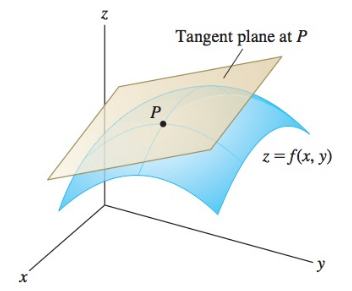
\includegraphics[width=.4\textwidth]{Figures/tangent-planes-1.png}
        \end{figure}
                
        \end{ex}
        
        \begin{ex}{Tangent Vectors}{tangent_vectors}
        Another way to understand this is to compute the \emph{tangent vectors} at a point. Take the same function $f(x,y)=-x^2-y^2$ and compute
        \begin{align*}
            \frac{\partial}{\partial x}\begin{bmatrix} x \\ y \\ f(x,y)\end{bmatrix} &= \begin{bmatrix} 1\\ 0 \\ -2x\end{bmatrix}\\
            \frac{\partial}{\partial y}\begin{bmatrix} x \\ y \\ f(x,y)\end{bmatrix} &= \begin{bmatrix} 0\\ 1 \\ -2y\end{bmatrix}.
        \end{align*}
        Then take the cross product of these two vectors to get the normal vector to the tangent plane
        \[
        \begin{bmatrix} 1 \\ 0 \\-2x\end{bmatrix} \times \begin{bmatrix} 0 \\ 1 \\ -2y\end{bmatrix} = \begin{bmatrix} 2x \\ 2y \\ 1\end{bmatrix}.
        \]
        Pick a point $(x_0,y_0)$ and the normal to tangent plane is given by
        \[
        \mathbf{n}=\begin{bmatrix} 2x_0 \\ 2y_0 \\ 1 \end{bmatrix}.
        \]
        Which leads us to the following equation of a plane (but not exactly the tangent plane)
        \[
        2x_0 x + 2y_0y+z=0.
        \]
        This plane is parallel to the tangent plane and is often a nicer tool.
        \end{ex}
        
        \begin{exercise}
        Take the two equations for the planes above and simplify each to having a zero right hand side.  Then subtract each of these equations from each other and see what the difference is.
        \end{exercise}
        
        
    \chapter{Calculus with Vector Fields}
        \section{The Jacobian of a Vector Field}
        Recall we can define a three dimensional vector field $\mathbf{v}(x,y,z)$ by
        \[
        \mathbf{v}(x,y,z)=(v_1(x,y,z),v_2(x,y,z),v_3(x,y,z)) = \begin{bmatrix} v_1(x,y,z) \\ v_2(x,y,z) \\ v_3(x,y,z) \end{bmatrix}
        \]
        where we call each $v_1$, $v_2$, and $v_3$ the component functions.  Notice that each component function is a scalar function!
        
        Since each component function is a scalar function, we know how to compute the derivative of each by computing the gradient.  This gives us a way to then talk about the derivative of the vector field as a whole
        
        \begin{df}{Jacobian}{jacobian}
        The \textbf{Jacobian} of a vector field $\mathbf{v}(x,y,z)$ is a matrix
        \[
        J(x,y,z)\coloneqq \begin{bmatrix} \nabla v_1^T \\ \nabla v_2^T \\ \nabla v_3^T \end{bmatrix},
        \]
        where the gradients are transposed (the superscript $T$) so they are are written as row vectors and placed in a matrix. More specifically, we can write this matrix as 
        \[
        J(x,y,z) = \begin{bmatrix} \frac{\partial v_1}{\partial x} & \frac{\partial v_1}{\partial y} & \frac{\partial v_1}{\partial z}\\ \frac{\partial v_2}{\partial x} & \frac{\partial v_2}{\partial y} & \frac{\partial v_2}{\partial z} \\ \frac{\partial v_3}{\partial x} & \frac{\partial v_3}{\partial y} & \frac{\partial v_3}{\partial z} \end{bmatrix}.
        \]
        \end{df}
        
        The Jacobian contains a lot of information. Intuitively, it tells us how each component of the vector field changes in each direction.  
        
        \begin{ex}{Computing the Jacobian, 1}{computing_jacobian}
        Let us consider the vector field
        \[
        \mathbf{v}(x,y,z) = (x^2+y^2,z,x+y+z).
        \]
        Then we can write
        \begin{align*}
            v_1(x,y,z)&= x^2+y^2\\
            v_2(x,y,z)&= z\\
            v_3(x,y,z)&= x+y+z.
        \end{align*}
        So we compute the gradients of each
        \begin{align*}
            \nabla v_1 &= \begin{bmatrix} 2x \\ 2y \\ 0 \end{bmatrix}\\
            \nabla v_2 &= \begin{bmatrix} 0 \\ 0 \\ 1 \end{bmatrix}\\
            \nabla v_3 &= \begin{bmatrix} 1 \\ 1 \\ 1 \end{bmatrix}.
        \end{align*}
        So then the Jacobian is
        \[as
        J(x,y,z) = \begin{bmatrix} 2x & 2y & 0 \\ 0 & 0 & 1\\ 1 & 1 & 1 \end{bmatrix}.
        \]
        \end{ex}
        
        A related and important quantity comes in the form of the determinant of the Jacobian.  We've previously talked about the determinant of a matrix as telling us the (signed) scaling of volume of a linear transformation.  That is, for example, if we have
        \[
        A = \begin{bmatrix} 2 & 0 & 0\\ 0 & 2 & 0\\ 0 & 0 & 2 \end{bmatrix}
        \]
        then $\det(A)=8$ and we say that volumes of parallelopipeds are increased by a factor of $8$ in this case.  
        
        When you are given a vector field, you can think of different regions of space being stretched differently.  This is why we have that the Jacobian is a matrix that depends on the position $(x,y,z)$.  In this case, the volumes that are being stretched are very very tiny parallelopipeds.  You can think of cubes with side lengths $dx$, $dy$, and $dz$. 
        
        \begin{ex}{Computing the Jacobian, 2}
        We found that given
        \[
        \mathbf{v}(x,y,z) = (x^2+y^2,z,x+y+z)
        \]
        that
        \[
        J(x,y,z) = \begin{bmatrix} 2x & 2y & 0 \\ 0 & 0 & 1 \\ 1 & 1 & 1 \end{bmatrix}
        \]
        As we can see, this matrix depends on position.  Let's compute the determinant
        \[
        |J(x,y,z)|=\det(J(x,y,z))=2(y-x). 
        \]
        Something weird seems to happen with $y=x$ as the determinant $|J(x,y,z)|$ will be zero in this case. Otherwise, things are fine.
        \end{ex}
        
        \section{Divergence and Curl}
        Often we do not need to use the whole Jacobian.  We will find it to be necessary for integration, however.  
        
        For analysis of vector fields, we often wish to break them into their smaller pieces.  Fundamentally, we can break vector fields into two parts:
        \begin{itemize}
            \item Sources and sinks,
            \item Rotations.
        \end{itemize}
        
        \subsubsection{Sources, Sinks, and Divergence Fields}
        With some vector fields, we can make the analogy that some quantity (think air or water) is being added or removed from the system.  We call these \emph{sources} and \emph{sinks} respectively.  We want to quantify how much of some quantity is being added. This quantity is called the \emph{divergence}.
        
        Recall, we can write
        \[
        \nabla = \begin{bmatrix} \frac{\partial}{\partial x} \\ \frac{\partial}{\partial y} \\ \frac{\partial}{\partial z} \end{bmatrix}.
        \]
        If we are also given a vector field
        \[
        \mathbf{v}(x,y,z) = \begin{bmatrix} v_1(x,y,z) \\ v_2(x,y,z) \\ v_3(x,y,z) \end{bmatrix},
        \]
        we can compute the \textbf{divergence} of $\mathbf{v}$ by
        \[
        \nabla \cdot \mathbf{v}(x,y,z) = \frac{\partial v_1}{\partial x} + \frac{\partial v_2}{\partial y} + \frac{\partial v_3}{\partial z}.
        \]
        Notice that this quantity is a scalar!  This scalar value, the divergence, tells us how much the vector field is diverging at a point $(x,y,z)$. In other words, it tells us how much of a quanitity is being added or removed there.
        
        \begin{ex}{Source Field}{source_field}
        Consider
        \[
        \mathbf{v}(x,y,z) = \begin{bmatrix} x \\ y \\ z \end{bmatrix}.
        \]
        Then the divergence is
        \[
        \nabla \cdot \mathbf{v}(x,y,z) = \frac{\partial v_1}{\partial x} + \frac{\partial v_2}{\partial y} + \frac{\partial v_3}{\partial z} = 1 + 1 + 1 = 3.
        \]
        We can think of a source of air being placed at each point that pumps in $3$ units of air per second, or specifically being pumped in at the origin. The vector field looks like:
        \begin{figure}[H]
            \centering
            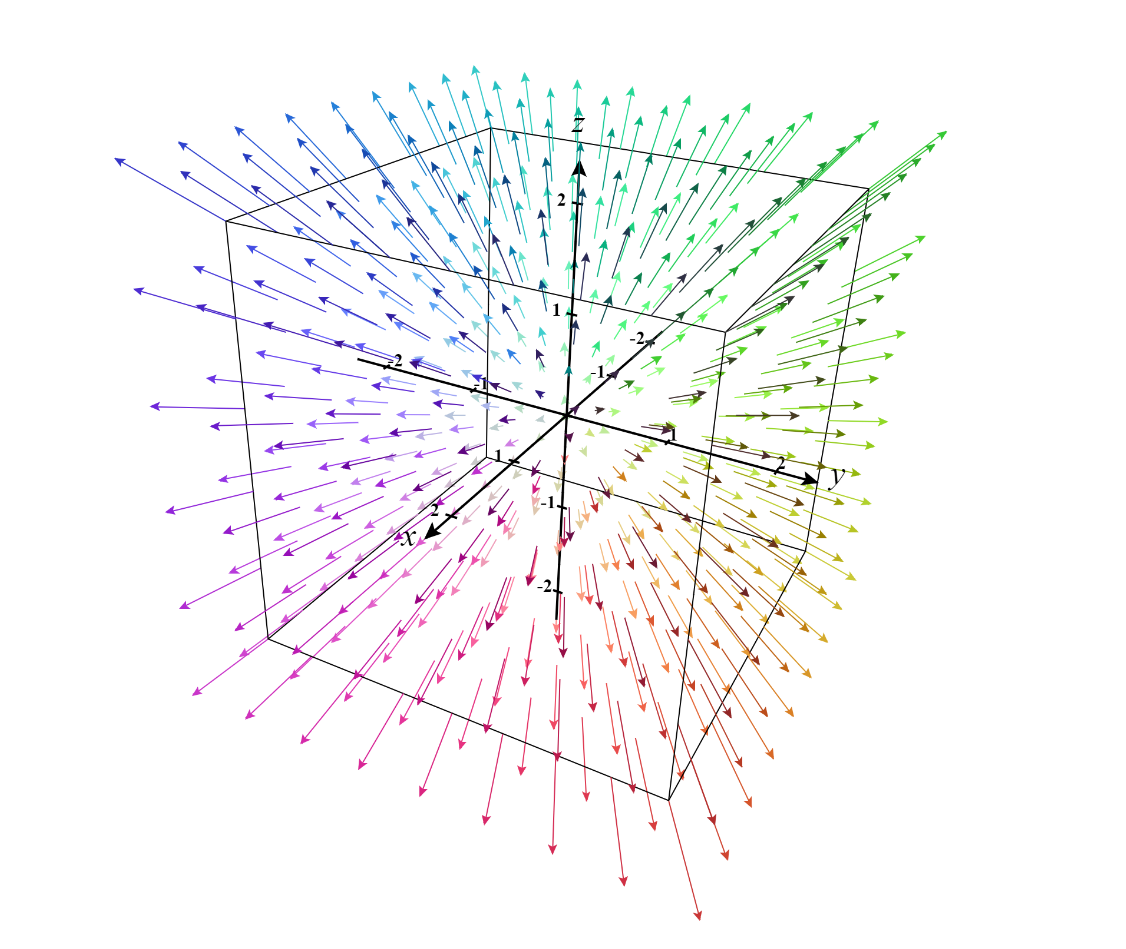
\includegraphics[width=.6\textwidth]{Figures/divergence_field.png}
        \end{figure}
        \end{ex}
        
        \subsubsection{Rotation Fields}
        The divergence was the quantity that measured the outflow from a point for a vector field.  The other quantity we can measure is the rotation of a vector field at a point.
        
        We define the \textbf{curl} of a vector field $\mathbf{v}(x,y,z)$ to be
        \[
        \nabla \times \mathbf{v}(x,y,z) = \begin{bmatrix} \frac{\partial v_3}{\partial y} - \frac{\partial v_2}{\partial z} \\ \frac{\partial v_1}{\partial z} - \frac{\partial v_3}{\partial x} \\ \frac{\partial v_2}{\partial x} - \frac{\partial v_1}{\partial y} \end{bmatrix}.
        \]
        \emph{Note that the curl is a vector!} The curl is a vector that points orthogonally to the plane where rotation occurs and has magnitude relative to how quickly the field swirls.
        
        It's a bit involved to go through the work and see exactly why this is the correct quantity for seeing rotation of a vector field.  However, you can recall that the cross product was useful in describing rotational motion of rigid bodies (that is, it showed up in angular velocity/momentum).
        
        \begin{ex}{A Rotation Field}{rot_field}
        Consider the vector field
        \[
        \mathbf{v}(x,y,z) = (-y,x,z)
        \]
        which looks like
        \begin{figure}[H]
            \centering
            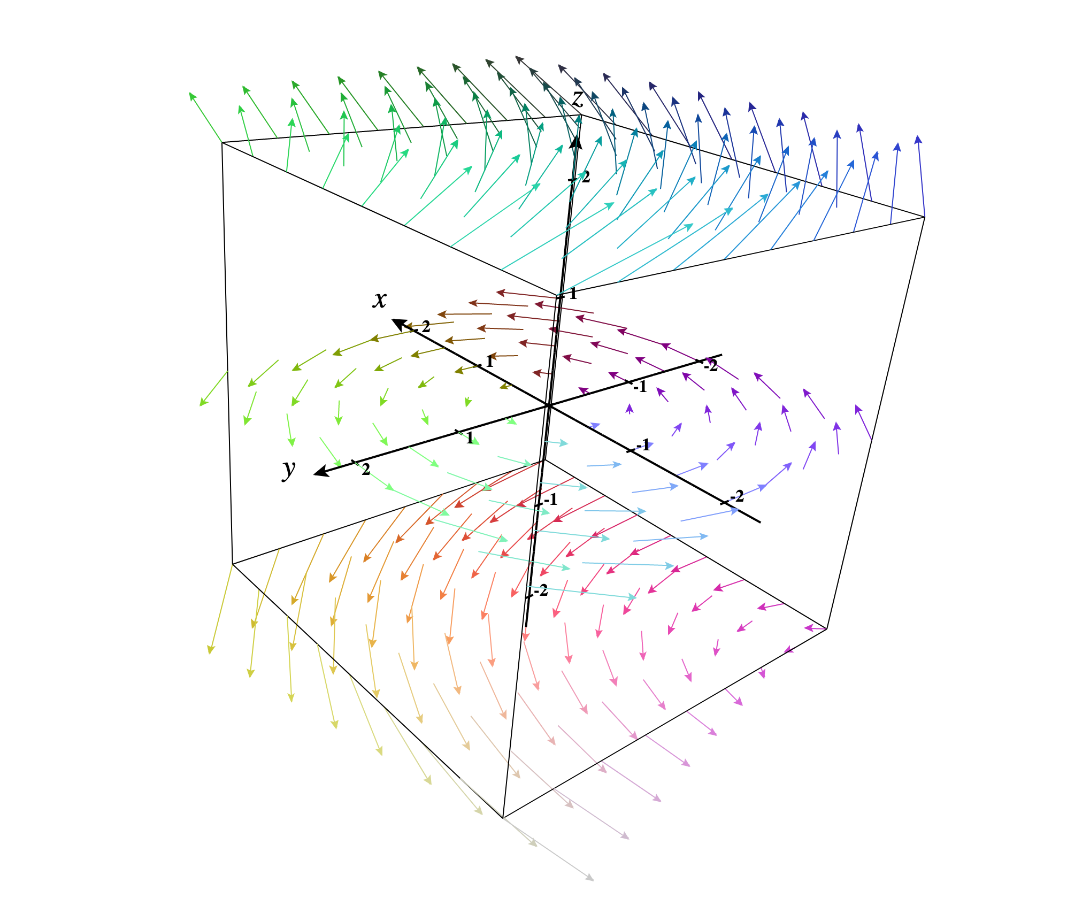
\includegraphics[width=.6\textwidth]{Figures/curl_field.png}
        \end{figure}
        We let
        \begin{align*}
            v_1(x,y,z) &= -y\\
            v_2(x,y,z) &= x\\
            v_3(x,y,z) &= z.
        \end{align*}
        If we look in this figure where $z=0$, we can clearly see that this field swirls around the origin.  If the curl is to measure rotation, we should see it nonzero here.
        
        Let us compute the curl of this field.  For this, we will all the other partial derivatives not contained in the divergence. That is, we need
        \begin{align*}
            \frac{\partial v_1}{\partial y} &= -1 & \frac{\partial v_1}{\partial z} &= 0\\
            \frac{\partial v_2}{\partial x} &= 1& \frac{\partial v_2}{\partial z} &= 0\\
            \frac{\partial v_3}{\partial x} &= 0 &  \frac{\partial v_3}{\partial y} &=0.
        \end{align*}
        Then we have
        \[
        \nabla \times \mathbf{v}(x,y,z) = \begin{bmatrix} 0-0\\ 0-0 \\ 1-(-1)\end{bmatrix} = \begin{bmatrix} 0\\ 0 \\ 2\end{bmatrix}.
        \]
        
        We can decipher the meaning here by saying that the swirling occurs in planes parallel to the $xy$-plane since the direction of the curl is only in the $z$-direction.  That is, curl is pointing perpendicularly to the plane of rotation.  How quickly the field swirls is given by the magnitude of the curl which is $2$ in this case.  Using the right hand rule we discussed previously this tells us the direction of swirling as well.  We have swirling counter-clockwise in the planes parallel to the $xy$-plane, and so we expect the curl to point in the positive $z$-direction.
        
        Take a moment to analyze this using the figure provided or by plotting this yourself.
        \end{ex}
        
        \begin{ex}{Divergence of the Rotation Field}
        One may also consider the divergent nature of the field 
        \[
        \mathbf{v}(x,y,z) = (-y,x,z)
        \]
        from the previous example and find that 
        \[
        \nabla \cdot \mathbf{v}(x,y,z) = 1.
        \]
        So, there is in some way divergence as well.  This leads us to breaking the vector field into a part that swirls and a part that diverges as follows:
        \begin{align*}
            \mathbf{v}_\textrm{swirl}(x,y,z) &= (-y,x,0)\\
            \mathbf{v}_\textrm{div}(x,y,z) &= (0,0,z).
        \end{align*}
        This type of analysis can be very helpful when considering real world problems.  It is especially important in electromagnetism.
        \end{ex}
        
        \subsubsection{Constant Vector Fields}
        Most of the understanding of vector fields was just covered by understanding the the part that diverges and the part that curls.  However, you can always add constants to these vector fields and these constants will not change the divergence or curl. Why? Take the following example.
        
        \begin{ex}{Constant Fields}{const_field}
        Let 
        \[
        \mathbf{v}(x,y,z) = (c_1,c_2,c_3)
        \]
        where $c_1,c_2,$ and $c_3$ are constants.  Then we can compute the Jacobian of $\mathbf{v}$
        \[
        J(x,y,z) = \begin{bmatrix} 0 & 0 & 0 \\ 0 & 0 & 0\\ 0 & 0 &0 \end{bmatrix}.
        \]
        Since the Jacobian holds all the partial derivative information, we can know from this that 
        \begin{align*}
            \nabla \cdot \mathbf{v} &= 0\\
            \nabla \times \mathbf{v} &= \mathbf{0}.
        \end{align*}
        \end{ex}
        
        \begin{exercise}
        Specifically show that the divergence and curl of a constant vector field (as in the previous example) are zero.  
        \end{exercise}
        
        All of this is to say that aside from the addition of a constant vector field, we understand the behavior by looking at divergence and curl.
        
        \section{The Laplacian of a Scalar Field}
        In the study of partial differential equations (PDEs), we are often asked to find a function $u(x,y,z)$ that satisfies the following equation
        \[
        \nabla \cdot \nabla u(x,y,z) = f(x,y,z)
        \]
        for some given function $f(x,y,z)$.  We will revisit this Part III, but for now we should see exactly what we mean by
        \[
        \nabla \cdot \nabla u(x,y,z).
        \]
        
        \begin{exercise}
        Show that
        \[
        \nabla \cdot \nabla u(x,y,z) = \frac{\partial^2 u}{\partial x^2} + \frac{\partial^2 u}{\partial y^2} + \frac{\partial^2 u}{\partial z^2}.
        \]
        \end{exercise}
        
        \begin{df}{Laplacian}{laplacian}
        We define the quantity
        \[
        \nabla \cdot \nabla u(x,y,z)
        \]
        to be the \textbf{Laplacian of $u(x,y,z)$} and we often write
        \[
        \Delta \coloneqq \nabla \cdot \nabla
        \]
        and call this the \textbf{Laplacian operator}.
        \end{df}
        
        Intuitively, the Laplacian can be summed up in a few ways. 
        \begin{itemize}
            \item The Laplacian is the \emph{divergence} of the \emph{gradient} of a scalar function.
            \item The Laplacian is the sum of ``curvatures" in each direction.
        \end{itemize}
        
        \begin{ex}{Computing the Laplacian}{compute_laplacian}
        Let us consider the functions
        \[
        f(x,y) = x^2+y^2
        \]
        and
        \[
        g(x,y) = x^2-y^2.
        \]
        Then we can compute the gradients of each function to get
        \begin{align*}
            \nabla f(x,y) &= \begin{bmatrix} 2x \\ 2y \end{bmatrix}\\
            \nabla g(x,y) &= \begin{bmatrix} 2x \\ -2y \end{bmatrix}.
        \end{align*}
        We can then compute the divergence of each of these and find
        \begin{align*}
            \nabla \cdot \nabla f(x,y) &= 2+2 = 4\\
            \nabla \cdot \nabla g(x,y) &= 2-2 =0.
        \end{align*}
        Let us see what these two functions look like to get a bit of an intuitive feel.
        \begin{figure}[H]
            \centering
            \begin{subfigure}[h]{.45\textwidth}
            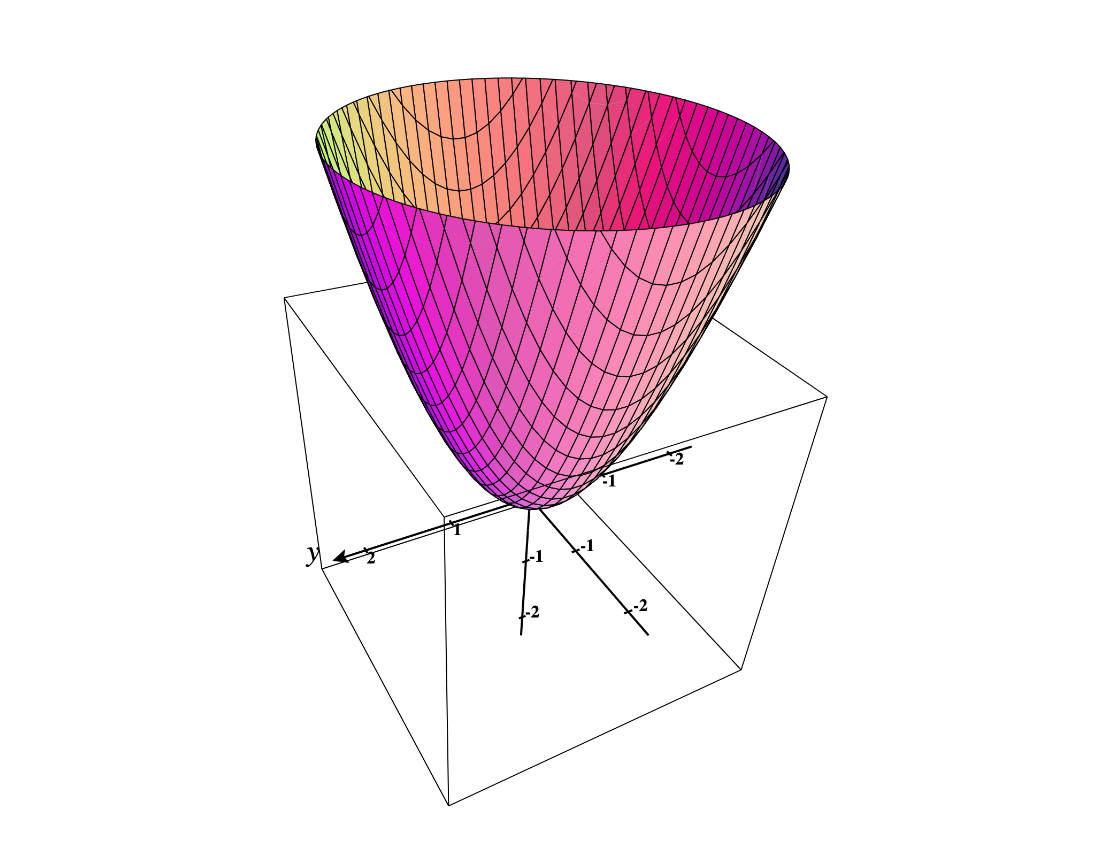
\includegraphics[width=\textwidth]{Figures/pos_laplace.png}
            \caption{A plot of $f(x,y).$}
            \end{subfigure}
            ~
            \begin{subfigure}[h]{.45\textwidth}
            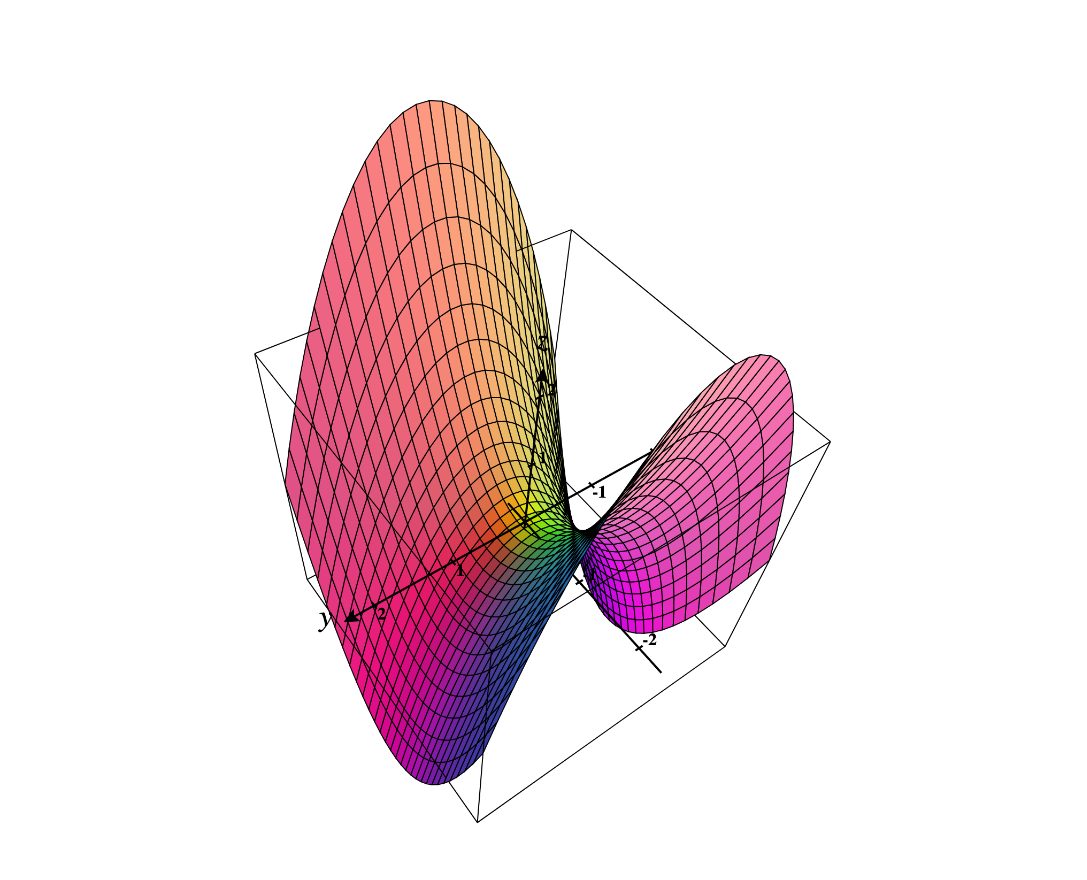
\includegraphics[width=\textwidth]{Figures/0_laplace.png}
            \caption{A plot of $g(x,y).$}
            \end{subfigure}
        \end{figure}
        Fundamentally we can see that these two functions are different.  It seems that for $f(x,y)$ we are curving upward in both the $x$ and $y$ direction which is what allows the Laplacian to be positive. However, for $g(x,y)$ one direction curves the opposite direction as the other which cancels out and gives us that the Laplacian is zero.  
        
        It turns out that the Laplacian describes many phenomenon. Two examples would be soap films and temperature flow.
        \end{ex}

        
        We have covered all of the differential calculus of multivariate functions that we need.  That does not mean it won't show up again, but the material won't be new.  We now move onto integration in multiple dimensions.
        
        \chapter{Integration in Multiple Dimensions}
        
        \section{Integration of Scalar Fields}
        
        \subsubsection{One Dimensional Case}
        In the case of one dimensional functions, we integrated to find the area under a curve.  That is, we were given a function $f(x)$ and asked to find
        \[
        \int_a^b f(x)dx
        \]
        which gave us the \emph{net} area under the curve.  Let's briefly review this with an example.
        
        \begin{ex}{One-Dimensional Integral}
        Let $f(x) = x^2+2$, $a=1,$ and $b=2$. Then we want to find
        \[
        \int_a^b f(x)dx = \int_1^2 x^2+2dx.
        \]
        Then we use the \emph{Fundamental Theorem of Calculus}. So, we find the antiderivative of the integrand and evaluate at the endpoints as follows
        \begin{align*}
            \int_1^2 x^2+2dx &= \left[ \frac{x^3}{3}+2x\right]_1^2\\
            &= \left(\frac{2^3}{3}+2(2)\right) - \left( \frac{1^3}{3}+2(1)\right)\\
            &= \frac{13}{3}.
        \end{align*}
        \end{ex}
        
        \subsubsection{Two Dimensional Case}
        
        Say we are now given a function $f(x,y)$ and bounds on both the $x$ and $y$ by
        $x_0 \leq x \leq x_1$ and $y_0 \leq y \leq y_1$.  We then wish to evaluate
        \[
        \int_{y_0}^{y_1} \int_{x_0}^{x_1} f(x,y)dxdy.
        \]
        You can think of this integral as being the \emph{net} volume under the surface given by $f(x,y)$.  
        
        How do we compute such an integral? The answer is iteratively.  Let's see how we do this with a concrete example.
        
        \begin{ex}{Two-Dimensional Integral}{2d_int}
        Let $f(x,y)=xy$, $x_0=1$, $x_1=2$, $y_0=3$ and $y_1=4$.  So, we want to evaluate
        \[
        \int_{y_0}^{y_1}\int_{x_0}^{x_1} f(x,y)dxdy = \int_3^4 \int_1^2 xy dxdy.
        \]
        The way we do this is by first evaluating the integral with respect to $x$ (holding $y$ constant) and then integrate with respect to $y$ ($x$ will not appear here). So, we integrate from the inside out.  
        
        Let's start by integrating with respect to $x$. We take
        \begin{align*}
            \int_1^2 xy dx &= \left[ \frac{x^2y}{2}\right]_1^2\\
            &= \left( y\frac{2^2}{2}\right) - \left(y\frac{1^2}{2}\right)\\
            &=\frac{3}{2}y.
        \end{align*}
        Now we take this function of $y$, and we integrate this with the bounds we are given.  
        \begin{align*}
            \int_3^4 \frac{3}{2}y dy &= \left[ \frac{3y^2}{4} \right]_3^4\\
            &= \frac{21}{4}.
        \end{align*}
        So we say that
        \[
        \int_3^4 \int_1^2 xy dxdy = \frac{21}{4}.
        \]
        
        Let's walk through the steps again. We did
        \begin{align*}
            \int_{y_0}^{y_1} \int_{x_0}^{x_1} f(x,y)dxdy&= \int_3^4\int_1^2 xy dxdy\\
            &= \int_3^4 \frac{3}{2}ydy \\
            &= \frac{21}{4}.
        \end{align*}
        \end{ex}
        
        \subsubsection{Three Dimensional Case}
        
        Integration here is performed in the same way.  We are given a function $f(x,y,z)$ and bounds on $x$, $y$, and $z$ such as $x_0\leq x \leq x_1$, $y_0\leq y\leq y_1$, and $z_0\leq z \leq z_1$. Then we evaluate
        \[
        \int_{z_0}^{z_1}\int_{y_0}^{y_1}\int_{x_0}^{x_1} f(x,y,z)dxdydz.
        \]
        Let's work through an example.
        
        \begin{ex}{Three-Dimensional Integral}{3d_int}
        Let
        \[
        f(x,y,z)=2x + 8xyz + 3,
        \]
        $x_0 = 0$, $x_1=1$, $y_0=2$, $y_1=3$, $z_0 =4$, $z_1=5$.  Then we want to find
        \[
        \int_{z_0}^{z_1}\int_{y_0}^{y_1}\int_{x_0}^{x_1} f(x,y,z)dxdydz = \int_4^5 \int_2^3 \int_0^1 2x+8xyz+3dxdydz.
        \]
        We do this iteratively.  So we first evaluate the $x$ integral holding the other variables constant for now.
        \begin{align*}
            \int_0^1 2x+8xyz+3 dx &= \left[ x^2 + 4x^2yz+3x\right]_0^1\\
            &= \left( 1^2 + 4(1)^2yz+3(1)\right) - \left( 0^2+4(0)^2yz+3(0)\right)\\
            &= 4yz+4.
        \end{align*}
        We then take this, and integrate with respect to $y$.
        \begin{align*}
            \int_2^3 4yz + 4 dy &= \left[ 2y^2z+4y\right]_2^3\\
            &= (4(3)^2z+4(3))-(4(2)^2z+4(2))\\
            &= 10z+4.
        \end{align*}
        Lastly, we integrate with respect to $z$
        \begin{align*}
            \int_4^5 10z+4 dz &= \left[ 5z^2+4z\right]_4^5\\
            &= (5(5)^2+4(5))-(5(4)^2+4(4))\\
            &=49.
        \end{align*}
        So we say that
        \[
        \int_4^5 \int_2^3 \int_0^1 2x+8xyz+3dxdydz = 49.
        \]
        Again, let's walk through the steps a bit
        \begin{align*}
            \int_{z_0}^{z_1}\int_{y_0}^{y_1}\int_{x_0}^{x_1} f(x,y,z)dxdydz &= \int_4^5 \int_2^3 \int_0^1 2x+8xyz+3dxdydz\\
            &= \int_4^5 \int_3^4 4yz+4dydz\\
            &= \int_4^5 10z+4dz\\
            &= 49.
        \end{align*}
        \end{ex}
        
        \section{Antiderivatives}
        In one variable calculus, we found that there is a relationship between the derivative and the indefinite integral.  In fact, this led us to call the indefinite integral the antiderivative.  This relationship was that
        \[
        \frac{d}{dx}\int f(x)dx = f(x)
        \]
        and
        \[
        \int \frac{df}{dx} = f(x) + C.
        \]
        From this, we realized that the indefinite integral is almost an inverse operation of the derivative.  It's just that in the case where we integrate a derivative, we only determine the function up to an additive constant. 
        
        \subsubsection{Potential Functions}
        The higher dimensional analog happens to be a bit more nuanced but the idea remains the same. Let's say we are given a function $f(x,y,z)$ and we compute, for example,
        \[
        \partialx.
        \]
        The issue now becomes this.  Let's say that we let
        \[
        f(x,y,z) = x+yz.
        \]
        Then we have that
        \[
        \partialx = 1.
        \]
        The terms with just a $y,z$ dependence disappear.  So if we were to try to undo this with an integral, we find that 
        \[
        \int \partialx dx = \int 1 dx = x + g(y,z).
        \]
        That is to say, when we take an indefinite integral a multivariate function with respect to one variable, there could be a function of the residual variables that we cannot determine!
        
        \subsubsection{Integrating the Gradient}
        
        Let's say that we are given $\mathbf{v}(x,y,z)=\nabla f(x,y,z)$ and are asked to find the original function $f(x,y,z)$.  This problem is called finding the \textbf{potential function} for $\mathbf{v}$.  Remember that
        \[
        \nabla f(x,y,z) = \begin{bmatrix} \partialx \\ \partialy \\ \partialz \end{bmatrix}.
        \]
        What we do is the following.
        \begin{enumerate}[1.]
            \item We integrate $\partialx$ with respect to $x$ and determine $f(x,y,z)$ up to adding a function of only $y$ and $z$.  That is we are able to recover what is essentially a third of the potential function $f(x,y,z)$.
            \item We integrate $\partialy$ with respect to $y$ and determine $f(x,y,z)$ up to adding a function of only $x$ and $z$.  
            \item We integrate $\partialz$ with respect to $z$ and determine $f(x,y,z)$ up to adding a function of only $x$ and $z$.
            \item Combine our knowledge from those three integrals we have determined $f(x,y,z)$ up to some additive constant!
        \end{enumerate}
        Let's work through an example.
        
        \begin{ex}{Finding a Potential Function}{find_potential}
        Let's say that we are given the gradient of some function
        \[
        \nabla f(x,y,z) = \begin{bmatrix} y+z \\ x+z \\ x+y \end{bmatrix}.
        \]
        Then we follow the steps above
        \begin{enumerate}[1.]
            \item We integrate $\partialx$ with respect to $x$.  So we have
            \begin{align*}
                \int y+z dx &= xy+xz + g(y,z).
            \end{align*}
            Here, $g(y,z)$ is a function of just $y$ and $z$ that we cannot determine yet.
            \item We integrate $\partialy$ with respect to $y$. So we have
            \begin{align*}
                \int x+z dy &= xy+yz + h(x,z).
            \end{align*}
            \item We integrate $\partialz$ with respect to $z$. So we have
            \begin{align*}
                \int x+y dz &= xz+yz + r(x,y).
            \end{align*}
            \item Now we know that all of these functions should be equal (up to a constant).  That is
            \[
            xy+xz+g(y,z)=xy+yz+h(x,z)=xz+yz+r(x,y).
            \]
            Here, we can see that $g(y,z)=yz$, $h(x,z)=xz$, and $r(x,y)=xy$.  So we have found that 
            \[
            f(x,y,z) = xy + xz + yz + C
            \]
            where the additive constant is there and is not something we can determine without a bit more information.
        \end{enumerate}
        \end{ex}
        
        \subsubsection{Requirements for Potentials}
        
        The main result here is the following.
        
        \begin{prop}{Curl of Gradient is Zero}{curl_of_gradient}
        We have that
        \[
        \nabla \times \nabla f(x,y,z) = \mathbf{0}
        \]
        for all $f(x,y,z)$.
        \end{prop}
        
        Then with a bit more work, one can show this follows.
       
       	\begin{thm}{Potential $\iff$ Curl Free}{potential_curl_free}
        Let $\mathbf{v}(x,y,z)$ be a vector field.  Then if 
        \[
        \nabla \times \mathbf{v} = \mathbf{0},
        \]
        then $\mathbf{v}(x,y,z) = \nabla f(x,y,z)$.  That is, a curl-free vector field $\mathbf{v}$ is really the gradient of some scalar function $f(x,y,z)$.  We call this scalar function $f$ the \textbf{potential} for $\mathbf{v}$.
        \end{thm}
        
        This is what allows one to define the \emph{voltage} in electrostatics.  When charges are not moving, we ave that the electric field $\mathbf{E}$ satisfies
        \[
        \nabla \times \mathbf{E} = \mathbf{0}
        \]
        and so it follows that
        \[
        \nabla V(x,y,z) = \mathbf{E}
        \]
        where $V$ is the potential.  We often call this electrostatic potential the voltage.